% Talk at High Throughput MD meeting in Barcelona
% Multiscale Modelling Group of Jun.-Prof. Birgit Strodel
% Given on November 08, 2013 at PPRB, Barcelona
%
% Oliver Schillinger

\documentclass[english]{beamer}

\usetheme{Juelich}
\usepackage[scaled]{helvet}

\usepackage[british]{babel}
\usepackage{graphicx,hyperref,url,color}
\usepackage{amsmath}
\usepackage[latin1]{inputenc}
\usepackage[T1]{fontenc} 
\usepackage{setspace}

%\usepackage[perpage,para,symbol]{footmisc}
%\renewcommand\footnotelayout{\tiny}
\usepackage{biblatex}
\bibliography{masterthesis}

\usepackage{ulem}

\setbeamercovered{transparent}
\setbeamertemplate{slide counter}[showall][]

\hypersetup{
    %bookmarks=false,        % show bookmarks bar?
    unicode=false,          % non-Latin characters in Acrobat’s bookmarks
    pdftoolbar=true,        % show Acrobat’s toolbar?
    pdfmenubar=true,        % show Acrobat’s menu?
    pdffitwindow=false,     % window fit to page when opened
    pdfstartview={FitH},    % fits the width of the page to the window
    pdftitle={Talk Masterthesis},    % title
    pdfauthor={Oliver Schillinger},     % author
    pdfsubject={Structure of Lipase-CitAP complex},   % subject of the document
    pdfcreator={Oliver Schillinger},   % creator of the document
    pdfproducer={Oliver Schillinger}, % producer of the document
    pdfkeywords={Lipase} {Citrate} {CitAP}, % list of keywords
    pdfnewwindow=true,      % links in new window
    colorlinks=true,        % false: boxed links; true: colored links
    linkcolor=black,          % color of internal links
    citecolor=green,        % color of links to bibliography
    filecolor=magenta,      % color of file links
    urlcolor=blue           % color of external links
}

% ============================================================================ %
%
% Multi column example
%
%\begin{frame}
%    \frametitle{Some title}
%    \framesubtitle{Some subtitle}
%
%    \begin{columns}[t]
%        \column{.5\linewidth}
%            Some text
%
%        \pause
%
%        \column{.5\linewidth}
%            Some more test
%
%    \end{columns}
%
%\end{frame}
%
% ============================================================================ % 

% Titlepage
\title[Masterthesis]{Masterthesis}
\subtitle[Structure]{Structure of Lipase-CitAP Complex\\
\textit{\small Supervisor: Jun.-Prof. Dr. Birgit Strodel}}
\author{Oliver Schillinger}
\institute{ICS-6 | Multiscale Modelling Group}
\date{8th November 2013} 

% ============================================================================ %

% begin document
\begin{document}

\maketitle

\begin{frame}
    \frametitle{Outline}
    \tableofcontents
\end{frame}

% ============================================================================ %

\section{Proteins}

\pagenumbering{arabic}

\begin{frame}
    \frametitle{Proteins}
    \framesubtitle{BsLA}

    \begin{columns}[t]
        \column{.6\linewidth}
        \begin{itemize}
            \item \textit{Bacillus subtilis} Lipase A
%            \item Minimal $\alpha/\beta$ hydrolase fold enzyme
            \item Structures down to 1.3 \r{A} resolution
            \item Catalyses hydrolysis and synthesis of \textbf{triacylgliycerols}
            \item Diverse substrate specificity
            \item Used in industry for
                \begin{itemize}
                    \item Resolution of racemic mixtures
                    \item Synthesis of esters
                    \item Additive laundry detergent
                \end{itemize}
        \end{itemize} 

        \column{.4\linewidth}
        \begin{figure}
            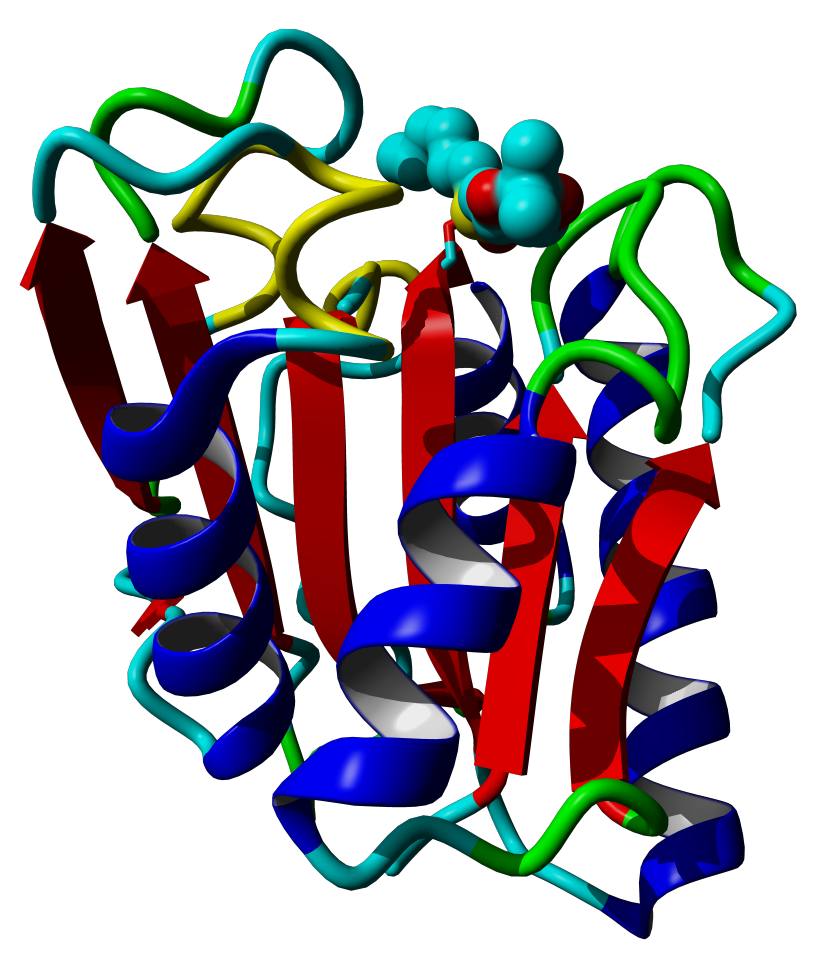
\includegraphics[width=.9\linewidth]{figures/Lipase.png}
        \end{figure}     
        \tiny Bacillus subtilis lipase A with covalently bound Rc-IPG-phosphonate inhibitor (PDB: 1R4Z)

    \end{columns} 

\end{frame}

% ============================================================================ %

%\begin{frame}
%    \frametitle{Proteins}
%    \framesubtitle{BsLA}
%
%    \begin{columns}[t]
%        \column{.6\linewidth}
%        \begin{itemize}
%            \item 181 amino acids
%            \item Much smaller than lipases from other organisms
%            \item Active site not covered by lid but solvent exposed -- \textbf{no interfacial activation} (activation due to lid opening in presence of lipid aggregates)
%        \end{itemize} 
%
%        \column{.4\linewidth}
%        \begin{figure}
%            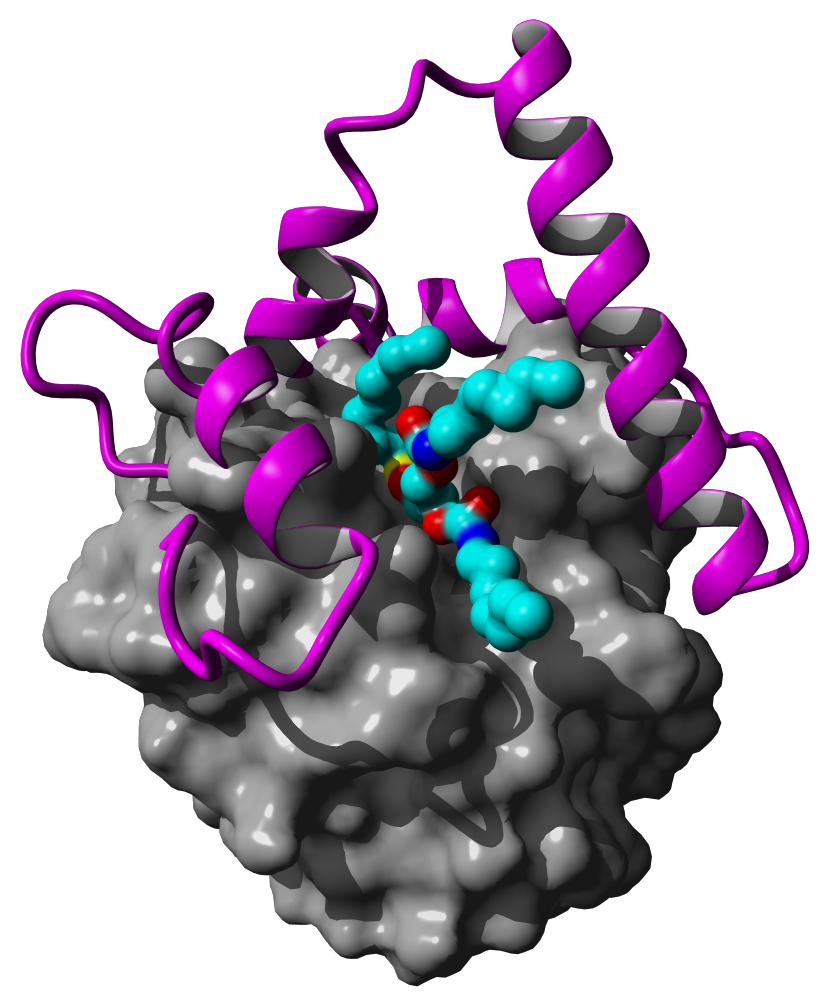
\includegraphics[width=\linewidth]{figures/Lipase_Lid.png}
%        \end{figure}     
%        \tiny BsLa lacks a lid covering the active site (Lid taken from P. Aeruginosa lipase, PDB: 1EX9)
%
%    \end{columns} 
%
%\end{frame} 

% ============================================================================ %

\begin{frame}
    \frametitle{Proteins}
    \framesubtitle{BsLA}

    \begin{columns}[t]
        \column{.5\linewidth}
        \begin{figure}
            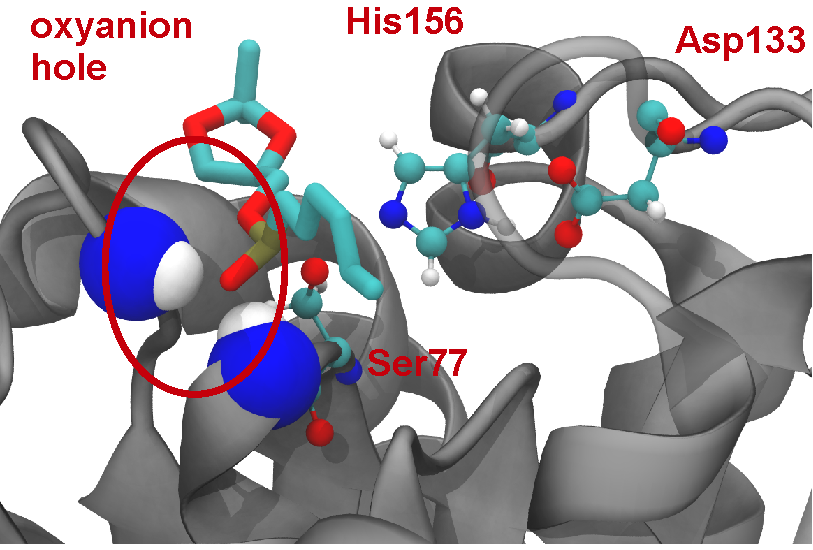
\includegraphics[width=1.0\textwidth]{figures/BSLA_pocket/BSLA_pocket_cartoon.pdf}
        \end{figure}      

        \column{.5\linewidth}
        \begin{figure}
            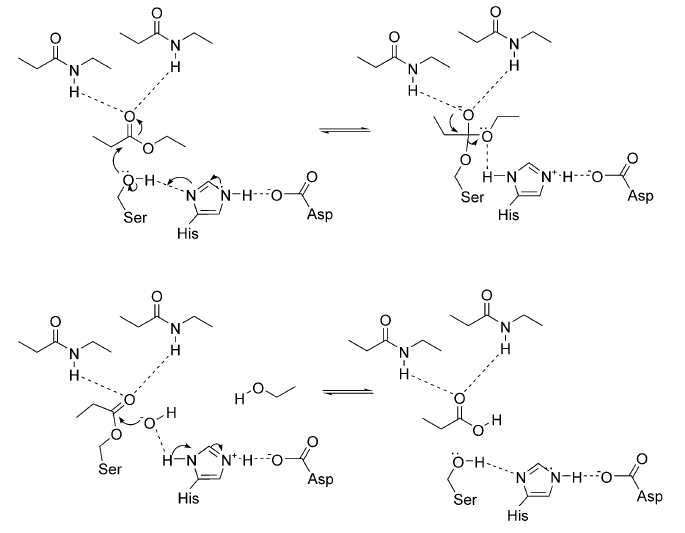
\includegraphics[width=1.0\textwidth]{figures/BSLA_reaction.png}
        \end{figure}     

    \end{columns} 

    \centering
    His156 -- Asp133 distance related to lipase activity

\end{frame}  

% ============================================================================ %

\begin{frame}
    \frametitle{Proteins}
    \framesubtitle{CitAP}

    \begin{itemize}
        \item Periplasmic domain of a two component system of a sensor and a response regulator
        \item CitA: Sensor Histidine Kinase
        \item CitB: is the corresponding response regulator
        \item \textit{Klebsiella pneumoniae} two component system is essential for the induction of citrate fermentation genes in the presence of citrate
    \end{itemize}
\end{frame} 

% ============================================================================ %

\begin{frame}
    \frametitle{Proteins}
    \framesubtitle{CitAP Signal Transduction Mechanism}
    \begin{figure}
        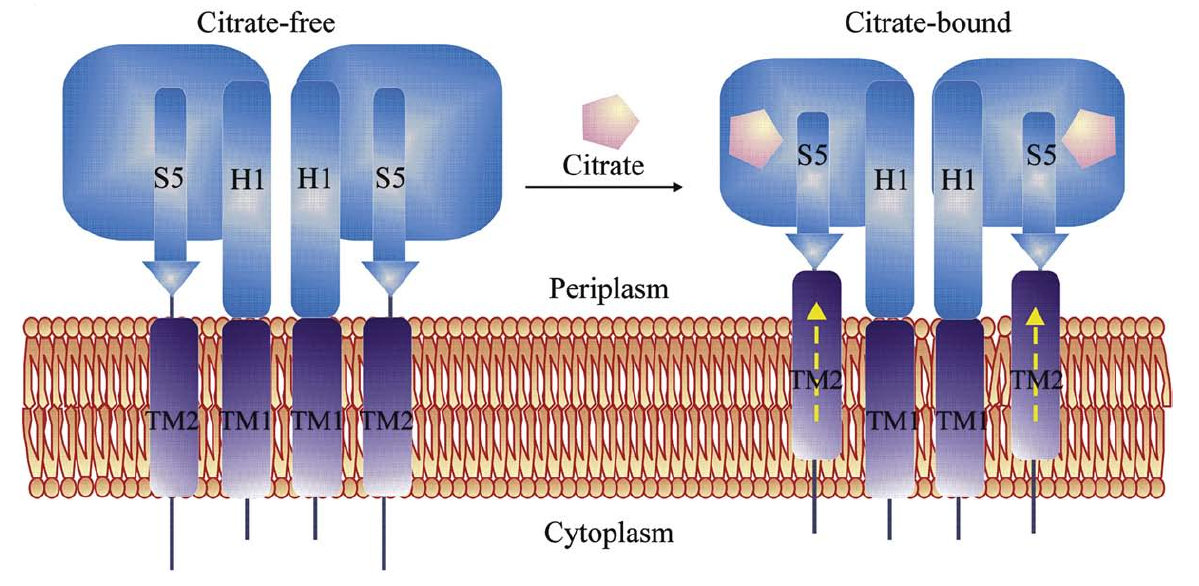
\includegraphics[width=.9\linewidth]{figures/CitA_mechanism.png}
    \end{figure}      

    \tiny
    \fullcite{CitA_2J80}

%    M. Sevvana, et. al,
%    \href{http://www.sciencedirect.com/science/article/pii/S0022283608000466}
%    {A Ligand--Induced Switch in the Periplasmic Domain of Sensor Histidine Kinase CitA},
%    \textit{J. Mol. Biol.}, 377, 512--523, 2008

\end{frame}  
 
% ============================================================================ %

%\begin{frame}
%    \frametitle{Proteins}
%    \framesubtitle{CitAP active site opening}
%    \begin{figure}
%        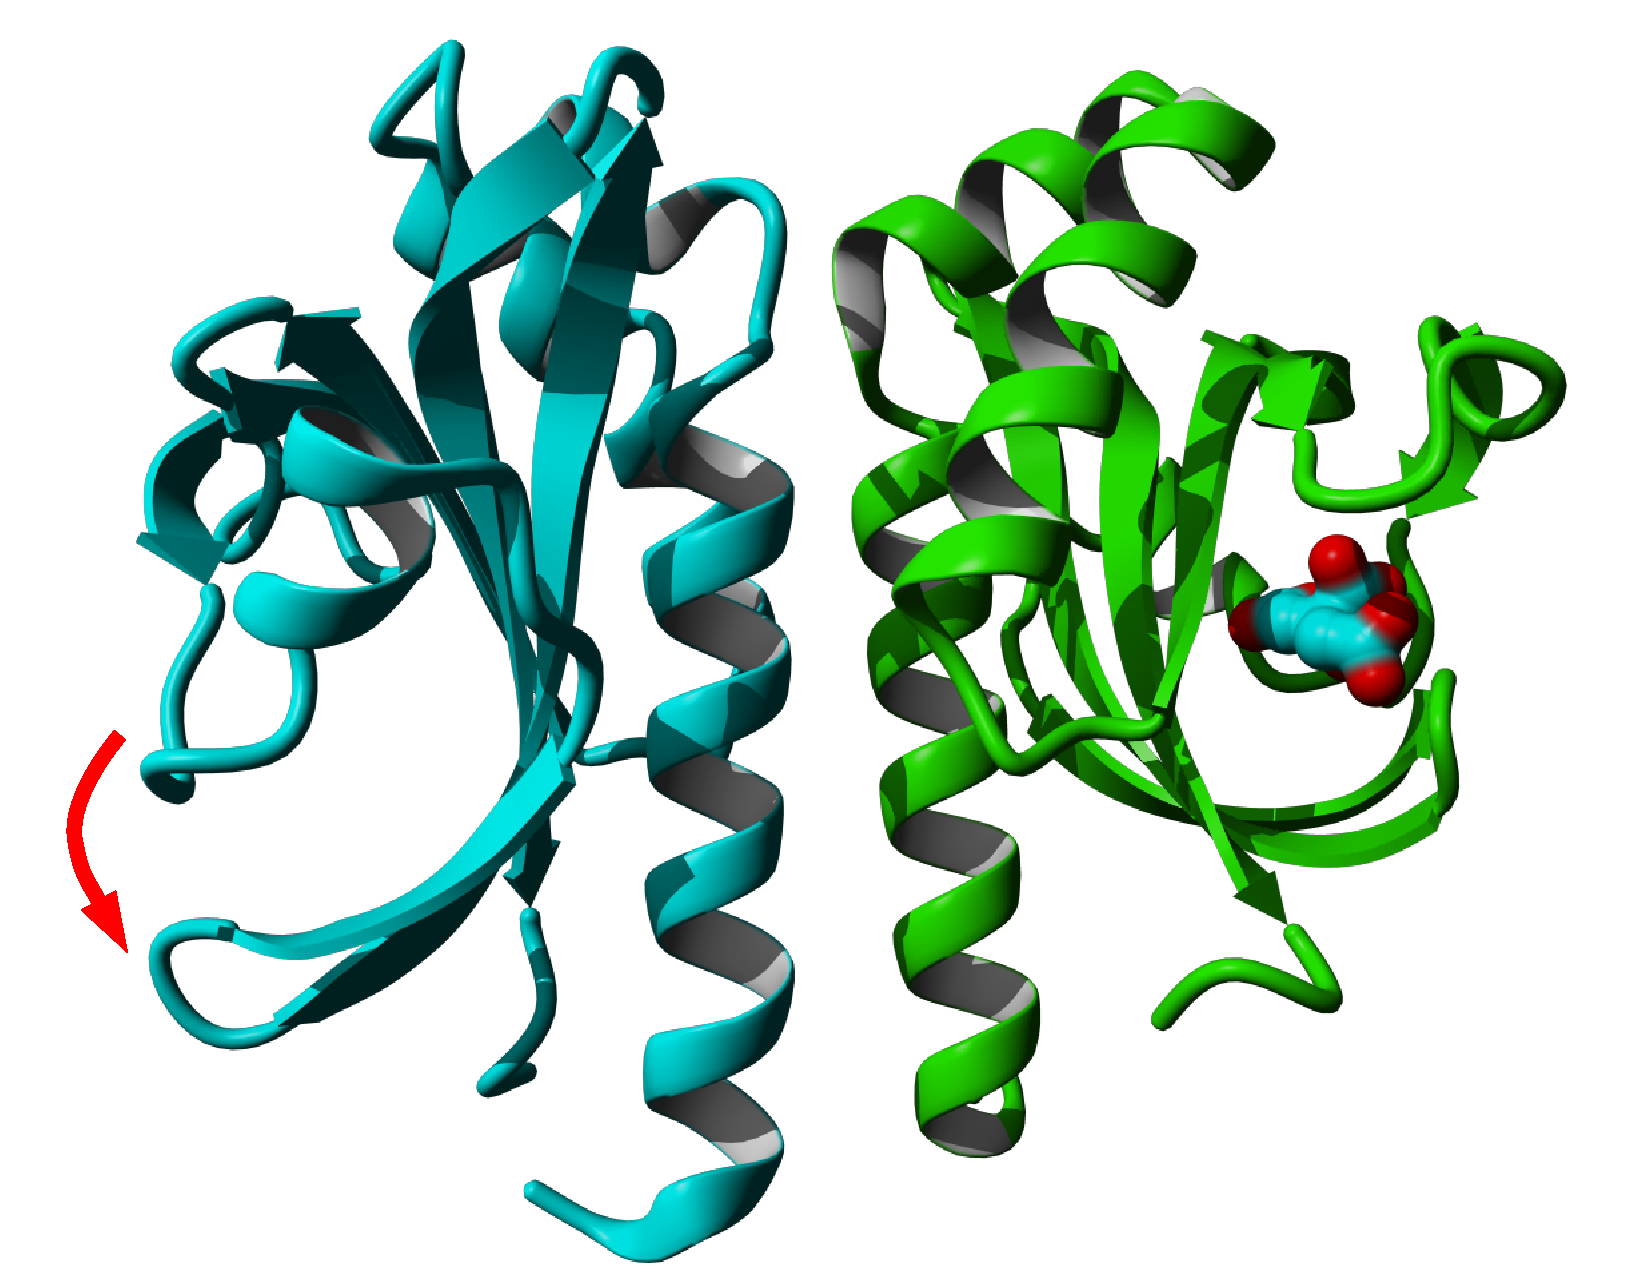
\includegraphics[width=.8\linewidth]{figures/CitA_dimer.pdf}
%    \end{figure}      
%
%\end{frame}   

% ============================================================================ %

\begin{frame}
    \frametitle{Proteins}
    \framesubtitle{CitAP Binding Pocket}

    \begin{figure}
        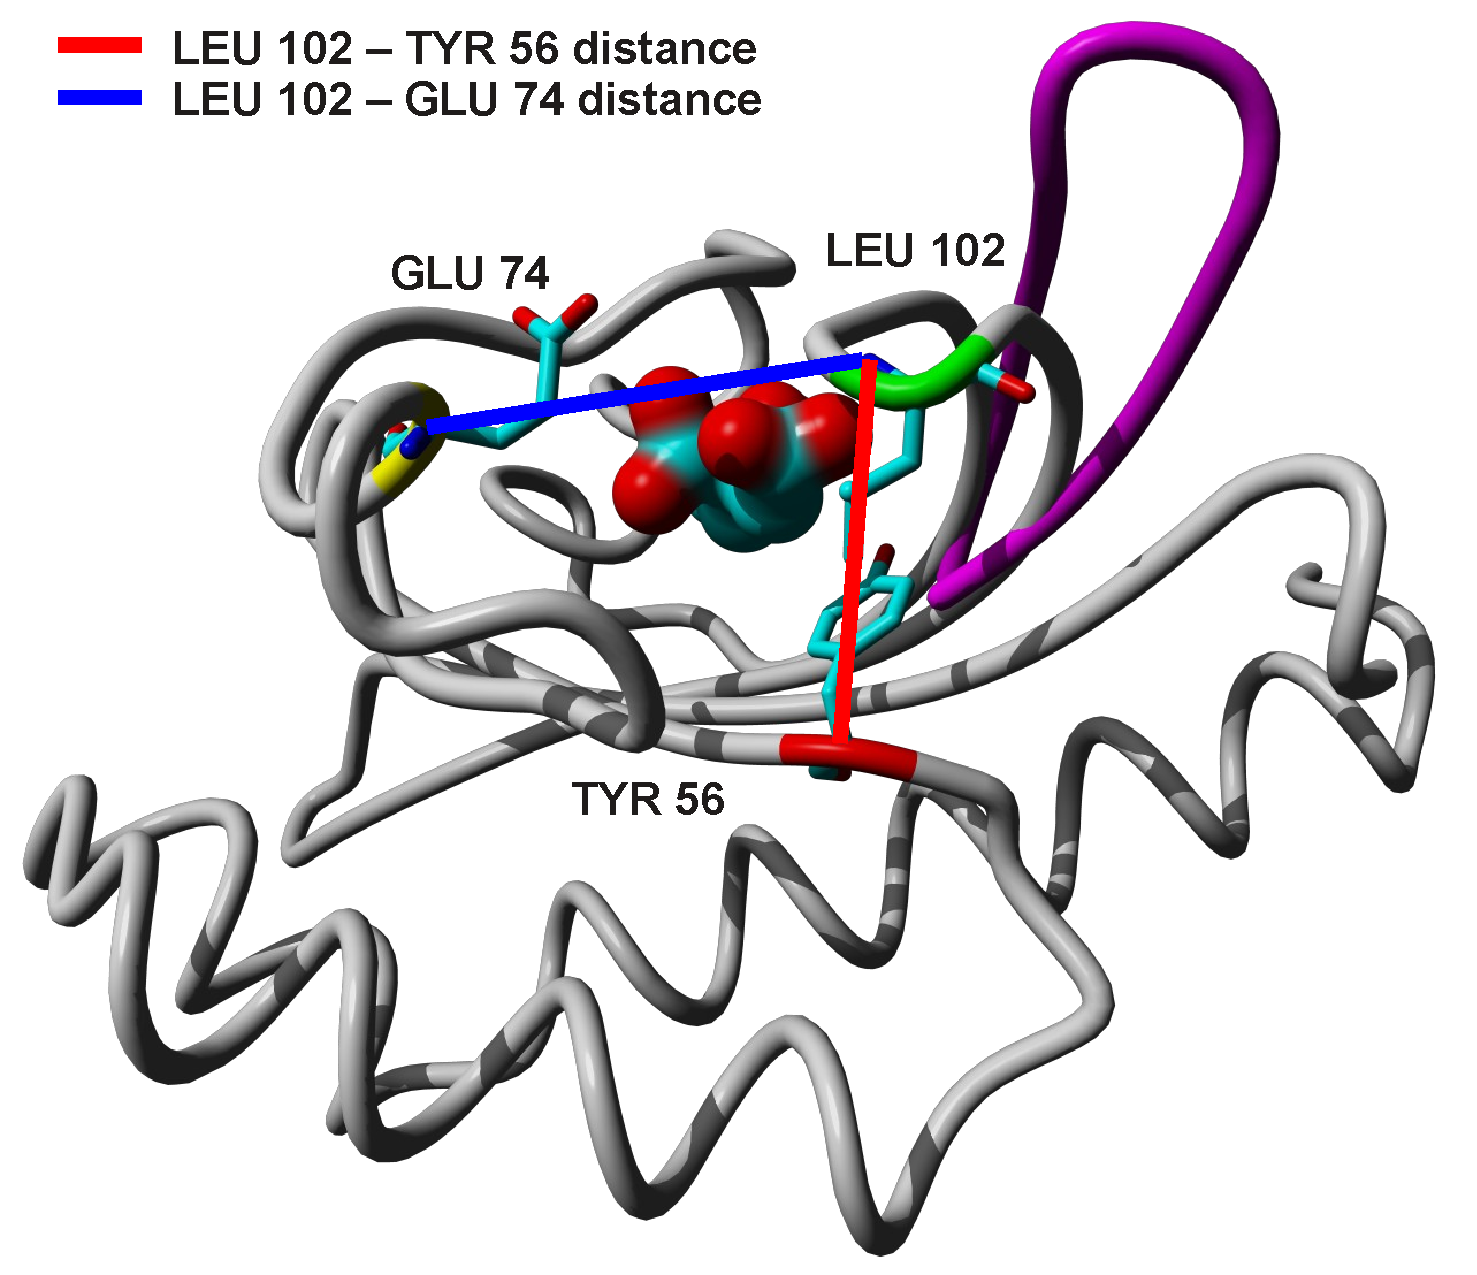
\includegraphics[width=.7\linewidth]{figures/CitA_pocket2.pdf}
    \end{figure}     
\end{frame}     

% ============================================================================ %

\begin{frame}
    \frametitle{Proteins}
    \framesubtitle{CitAP Citrate Interactions}

    \begin{figure}
        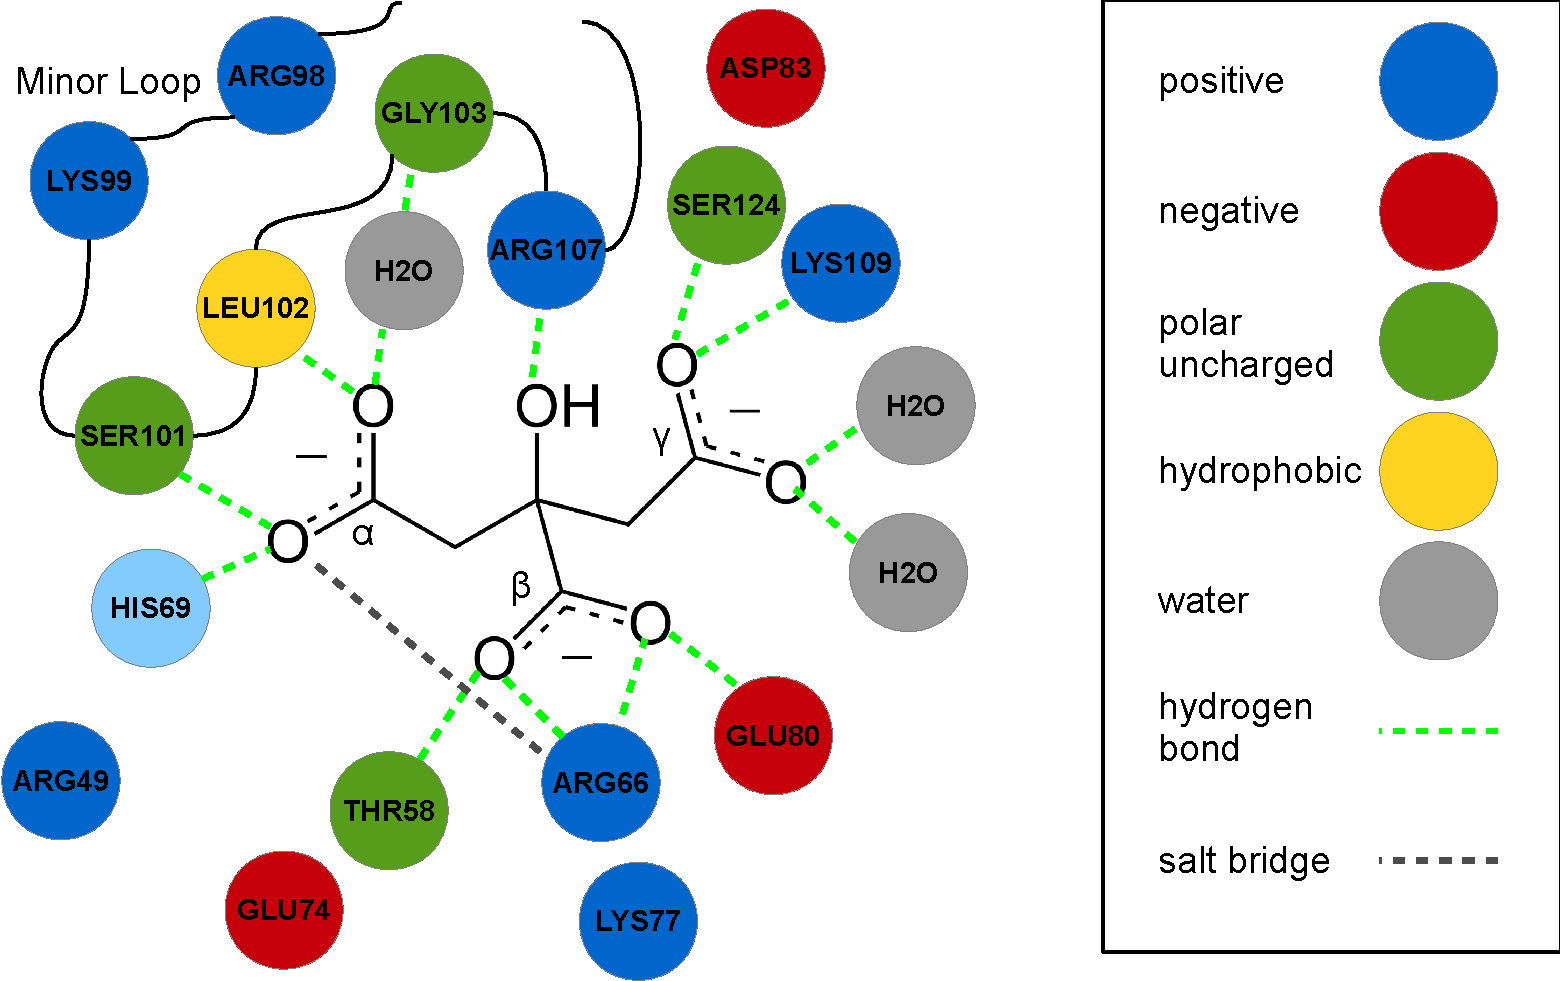
\includegraphics[width=0.9\textwidth]{figures/citrate_interactions/citrate_interactions.pdf}
    \end{figure}     
\end{frame}      

% ============================================================================ %

\begin{frame}
    \frametitle{Proteins}
    \framesubtitle{Complex}

    \setbeamercovered{invisible}

    \begin{block}{Why make a complex?}
        If citrate could trigger lipase activity we had a switchable detergent!
    \end{block}

    \pause

    \begin{columns}[t]
        \column{.88\linewidth} 
        \vspace{-3ex}
        \begin{figure}
            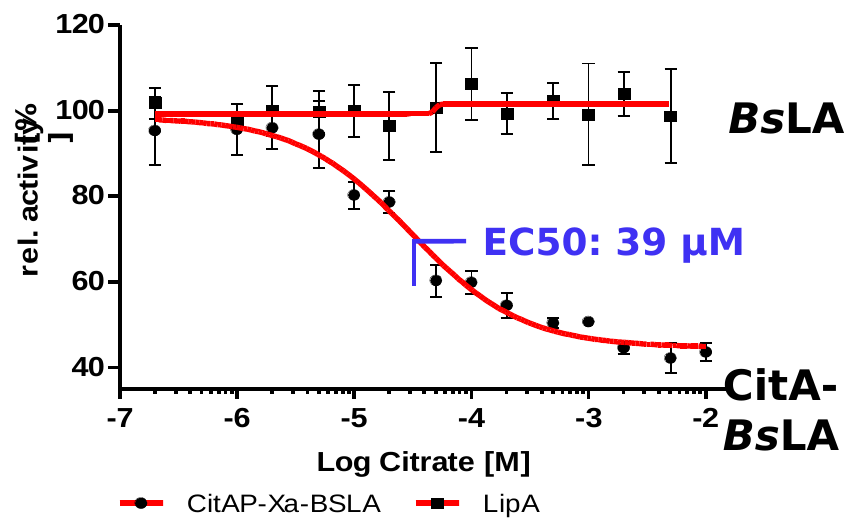
\includegraphics[width=0.7\textwidth]{figures/BSLA_activity/BSLA_activity.png}
        \end{figure}       
        \vfill

        \column{.12\linewidth} 
        \tiny
        Jaeger et al.
    \end{columns}

\end{frame}  

% ============================================================================ %

\begin{frame}
    \frametitle{Proteins}
    \framesubtitle{Complex}

    \begin{figure}
        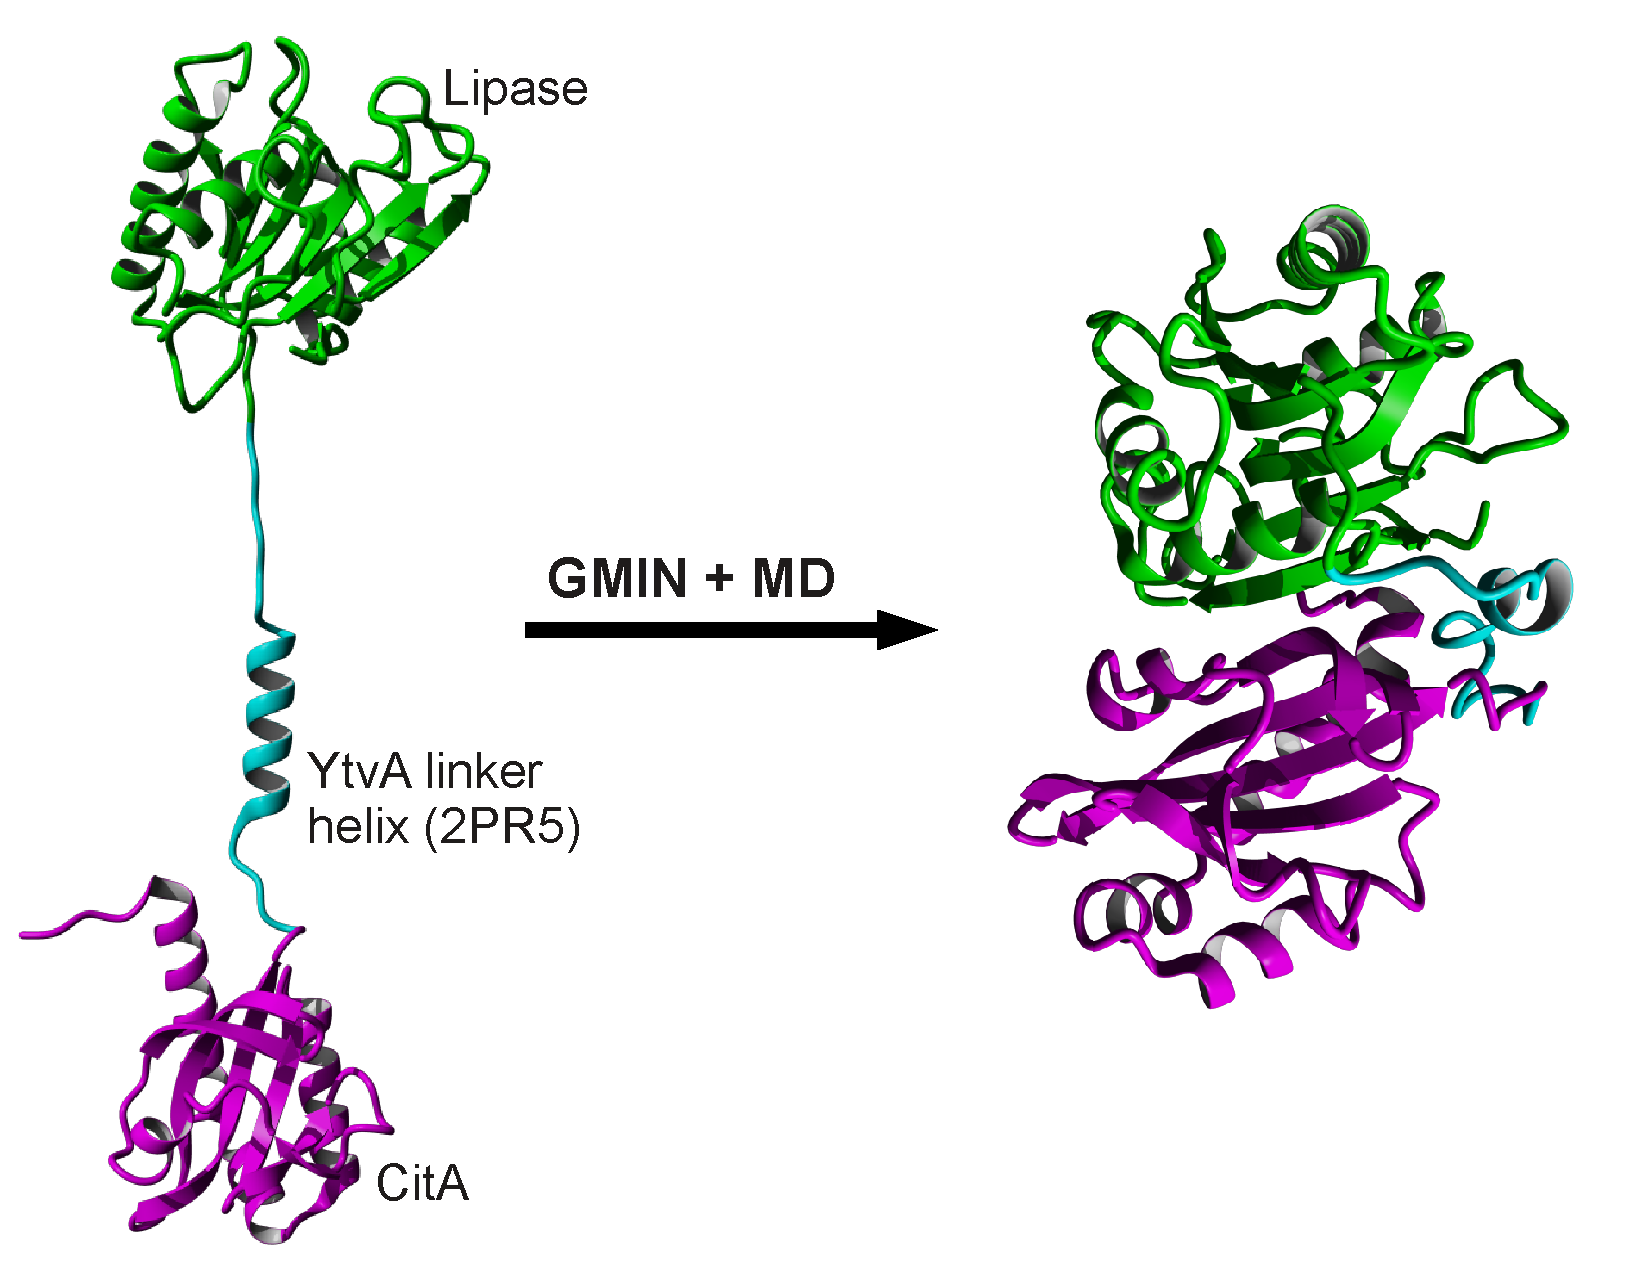
\includegraphics[width=.9\linewidth]{figures/complex/complex_folding.pdf}
    \end{figure}       

\end{frame}   

% ============================================================================ %

\section{Methods}

\begin{frame}
    \frametitle{Methods}
    \framesubtitle{MD} 

    \begin{itemize}
        \item GROMACS
        \item \textbf{\texttt{amber99sb-ildn-nmr}} force field
        \item 10 ns position restrained equilibration
        \item Gradually decreasing restraining force constant
        \item 100 ns production runs
        \item PBC, NPT, PME
        \item Mixed hardware: Clusters (up to 180 cores), GPUs (up to 4)
    \end{itemize}

\end{frame}    

% ============================================================================ %

\begin{frame}
    \frametitle{Methods}
    \framesubtitle{GMIN: Basin Hopping with Global Optimization}

    \begin{figure}
        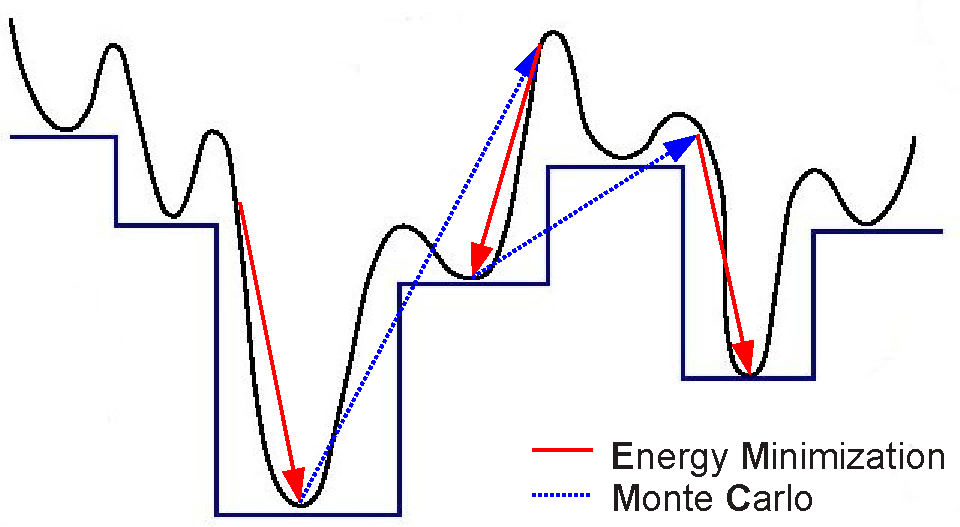
\includegraphics[width=0.9\textwidth]{figures/GMIN/GMIN.pdf}
    \end{figure}        

\end{frame}    


% ============================================================================ %

\begin{frame}
    \frametitle{Methods}
    \framesubtitle{Dimensionality Reduction}

    \begin{figure}
        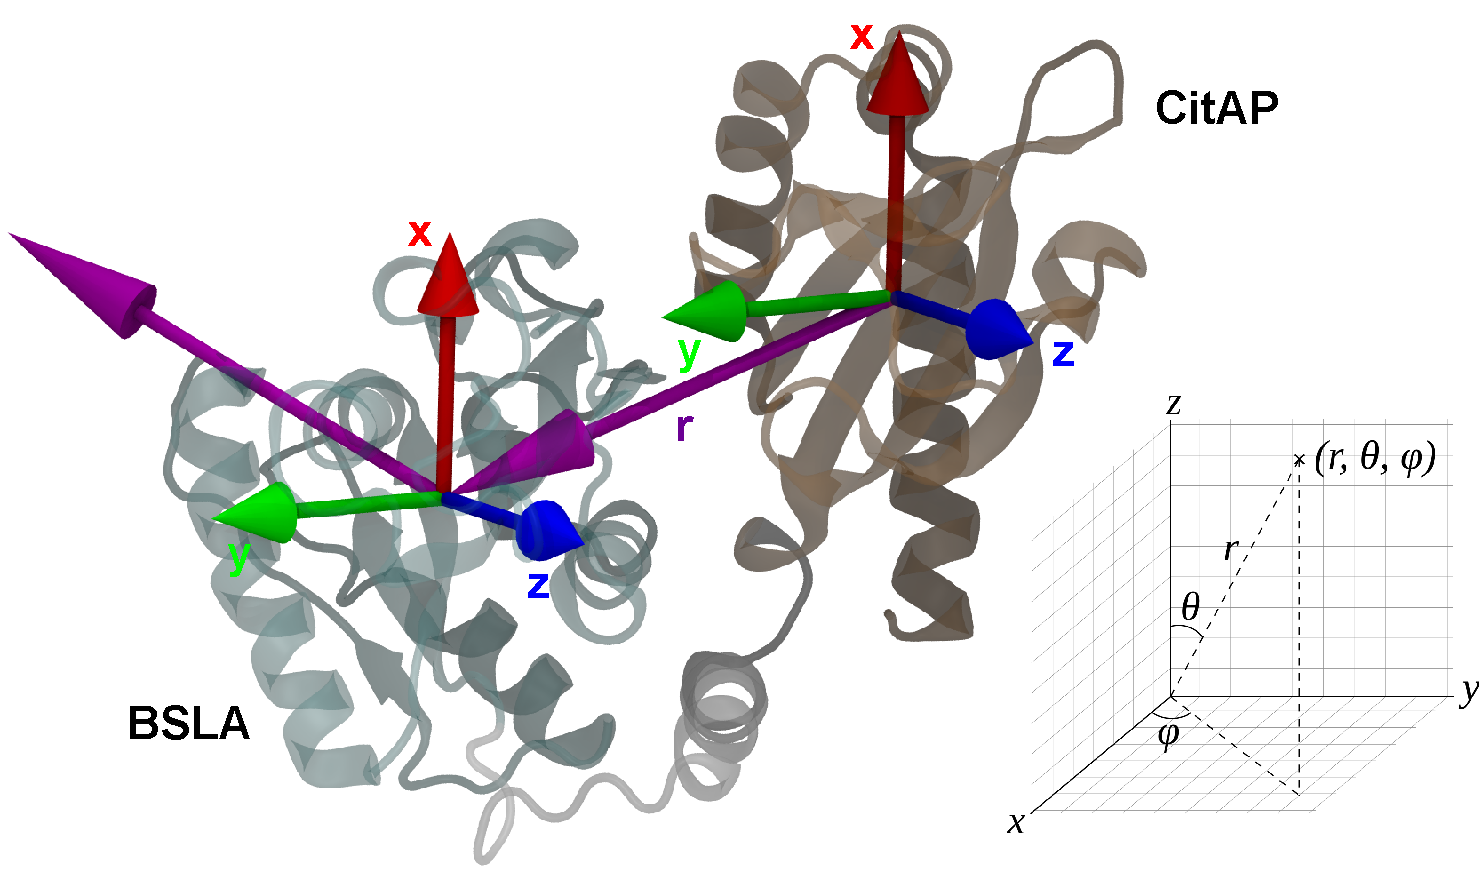
\includegraphics[width=1.0\textwidth]{figures/Collective_coords/collective_coords.pdf}
    \end{figure}        

\end{frame}     
 
% ============================================================================ %

\section{Results}

\begin{frame}
    \frametitle{Results}
    \framesubtitle{Solo CitAP Binding Pocket}

    \vspace{1.0\topmargin}

    \begin{figure}
        \hspace{0.2\textwidth}
        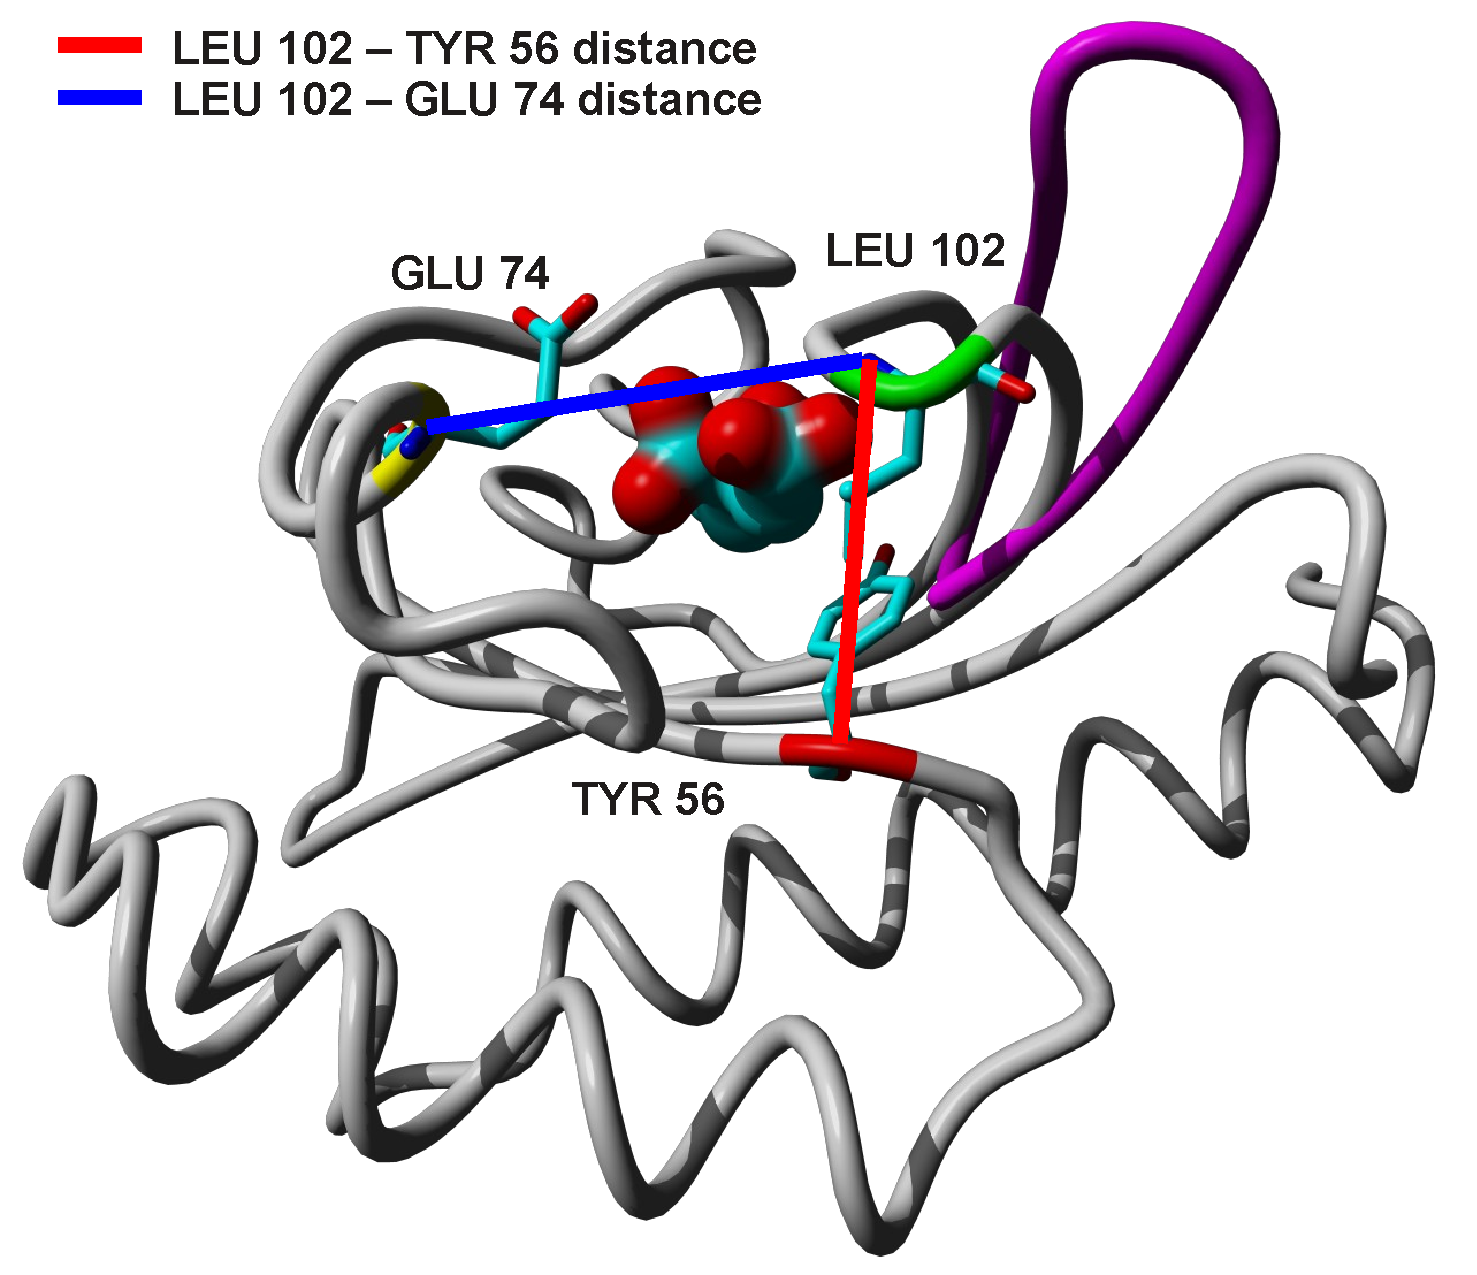
\includegraphics[width=.4\linewidth]{figures/CitA_pocket2.pdf}
    \end{figure}     

    \vspace{-1.2cm}

    \begin{columns}[t]
        \column{.5\linewidth} 
        \begin{figure}
            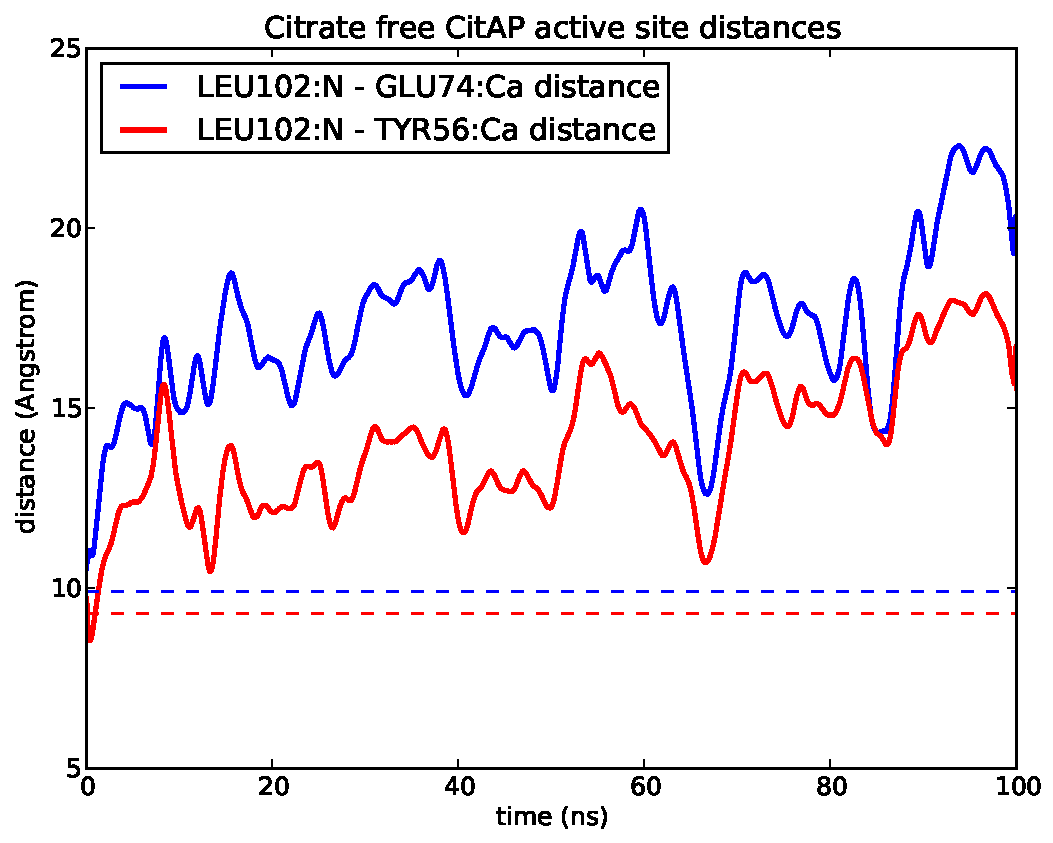
\includegraphics[width=1.0\textwidth]{figures/CitAP_opening/CitAP_dist_free.pdf}
        \end{figure}       

        \column{.5\linewidth} 
        \begin{figure}
            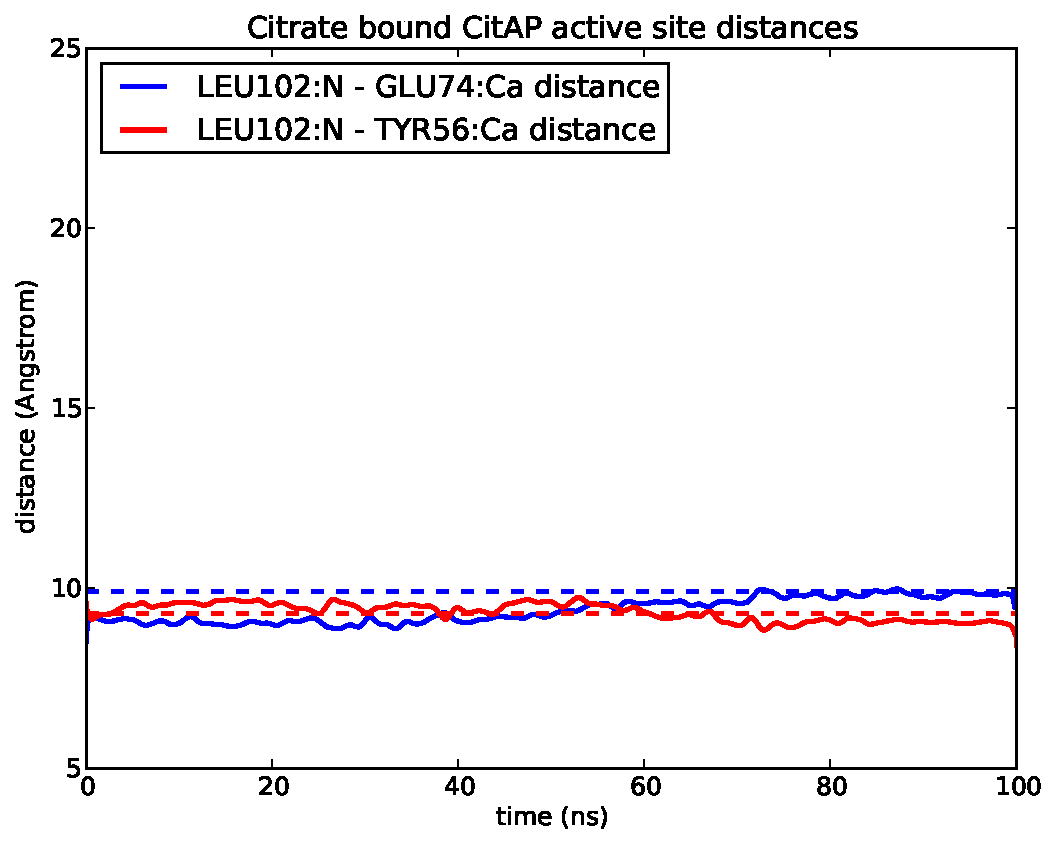
\includegraphics[width=1.0\textwidth]{figures/CitAP_opening/CitAP_dist_bound.pdf}
        \end{figure}        

    \end{columns} 


\end{frame}    

% ============================================================================ %

\begin{frame}
    \frametitle{Results}
    \framesubtitle{Solo BSLA MD} 

    \vspace{0.10\topmargin}

    \begin{figure}
        \begin{minipage}[t]{0.45\linewidth}
            \centering
            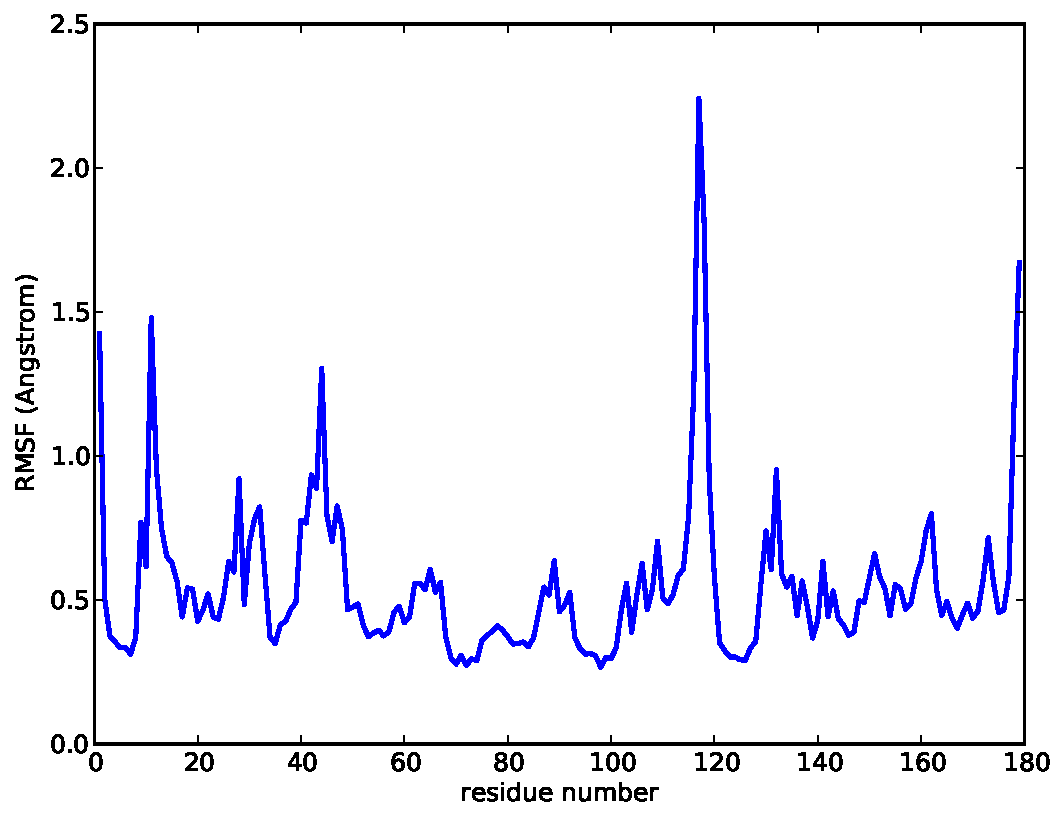
\includegraphics[width=1.0\textwidth]{figures/BSLA_solo/BSLA_solo_rmsf.pdf}  
            \linebreak
            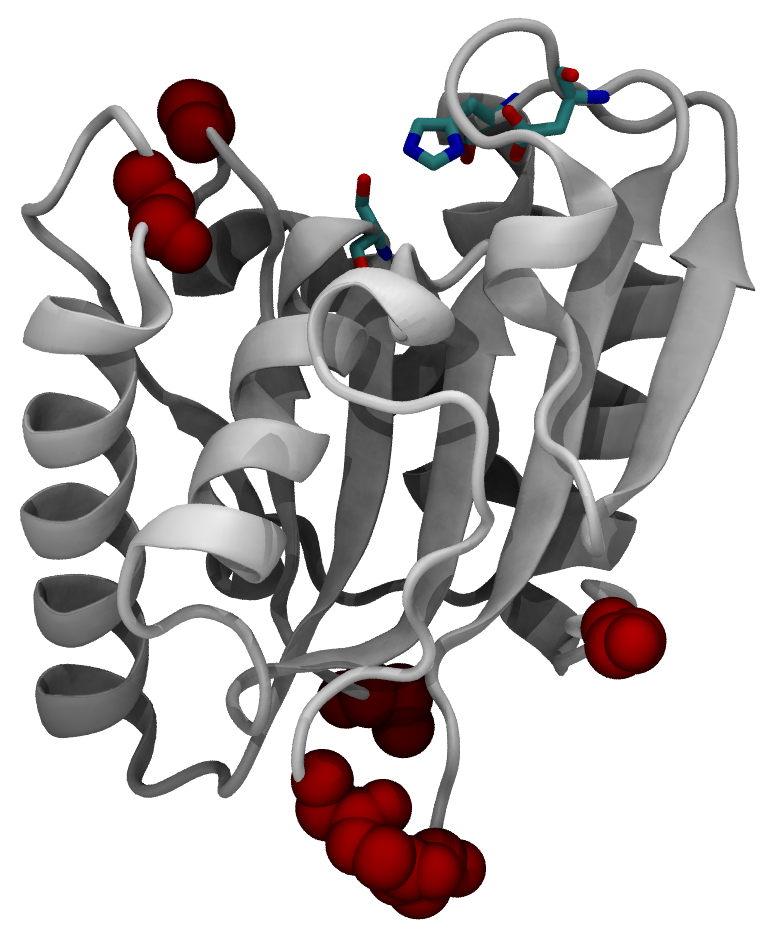
\includegraphics[width=0.65\textwidth]{figures/BSLA_flexibility.png}
        \end{minipage}
    \hspace{0.5cm}
        \begin{minipage}[t]{0.45\linewidth}
            \centering
            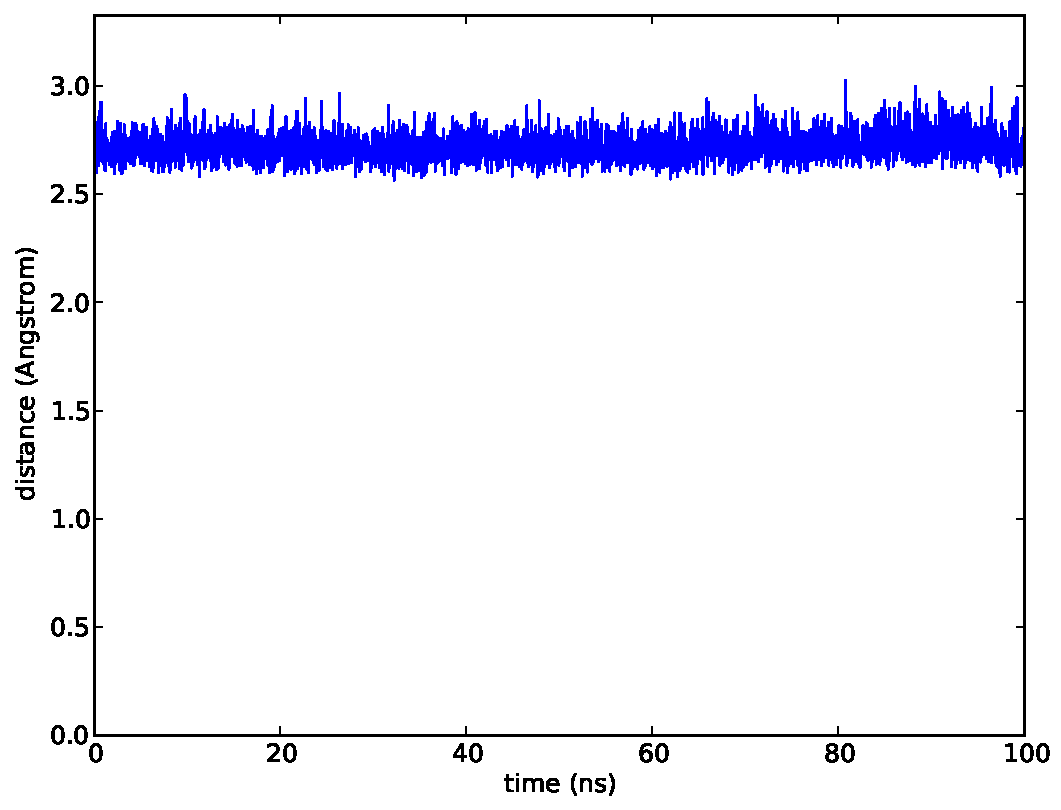
\includegraphics[width=1.0\textwidth]{figures/BSLA_solo/BSLA_solo_dist_ASP133_HIS156.pdf} 
            \linebreak
            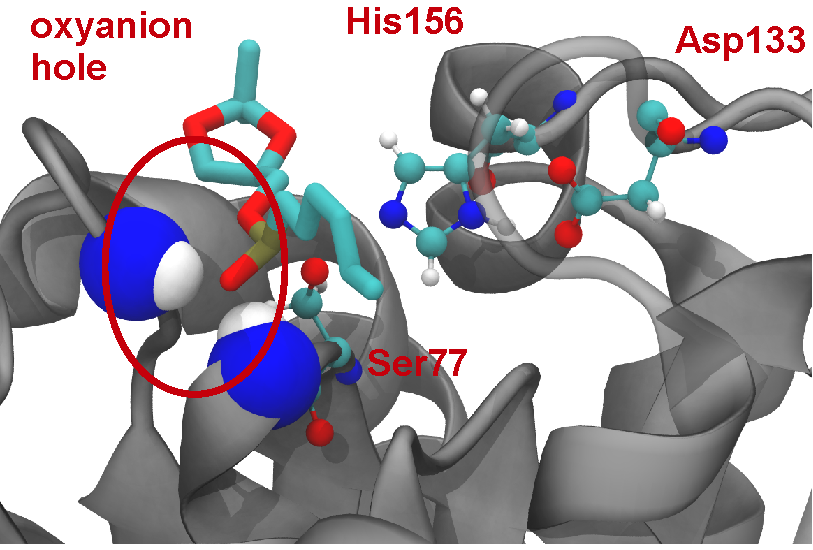
\includegraphics[width=1.0\textwidth]{figures/BSLA_pocket/BSLA_pocket_cartoon.pdf}
            %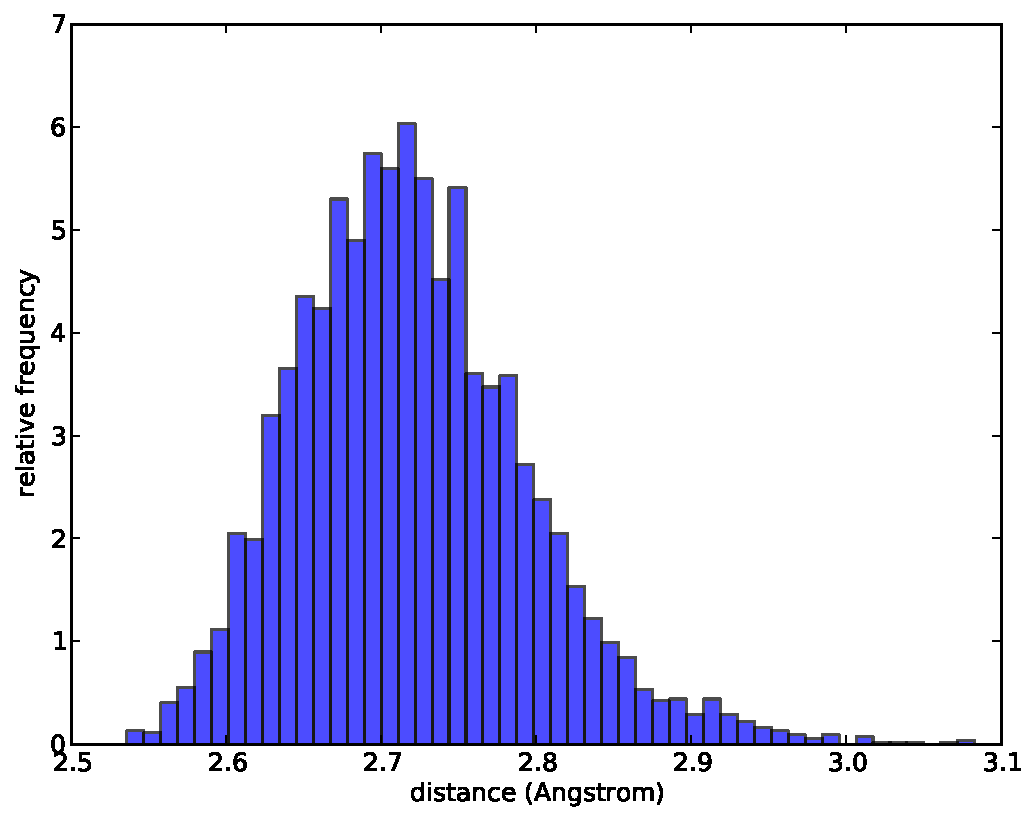
\includegraphics[width=0.9\textwidth]{figures/BSLA_solo/BSLA_distribution_ASP133_HIS156.pdf}  
        \end{minipage}
    \end{figure}  

\end{frame}    

% ============================================================================ %

\begin{frame}
    \frametitle{Results}
    \framesubtitle{GMIN Basin Hopping Structures} 

    \vspace{0.10\topmargin}

%    \begin{columns}[t]
%        \column{.5\linewidth}
%        \centering
%        Dimensionality Reduction
%        \begin{figure}
%            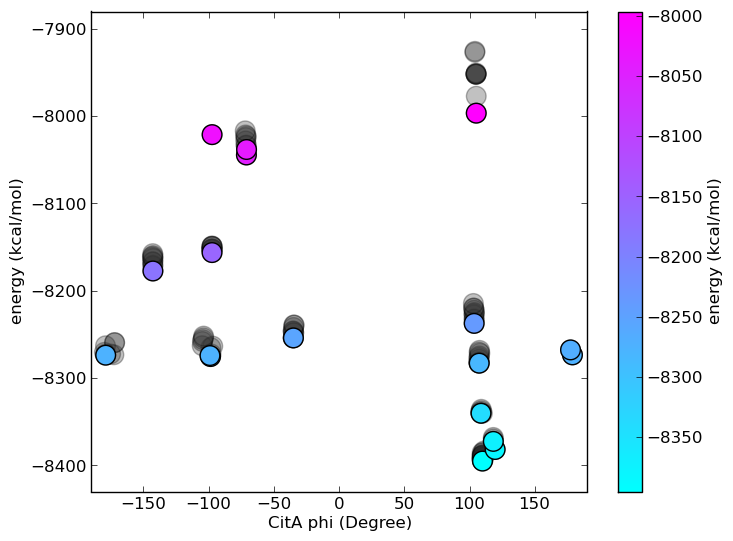
\includegraphics[width=1.0\textwidth]{figures/CitA_phi.png}
%        \end{figure}      
%
%        \column{.5\linewidth}
%        \centering
%        Basin Hopping Structures
%        \begin{figure}
%            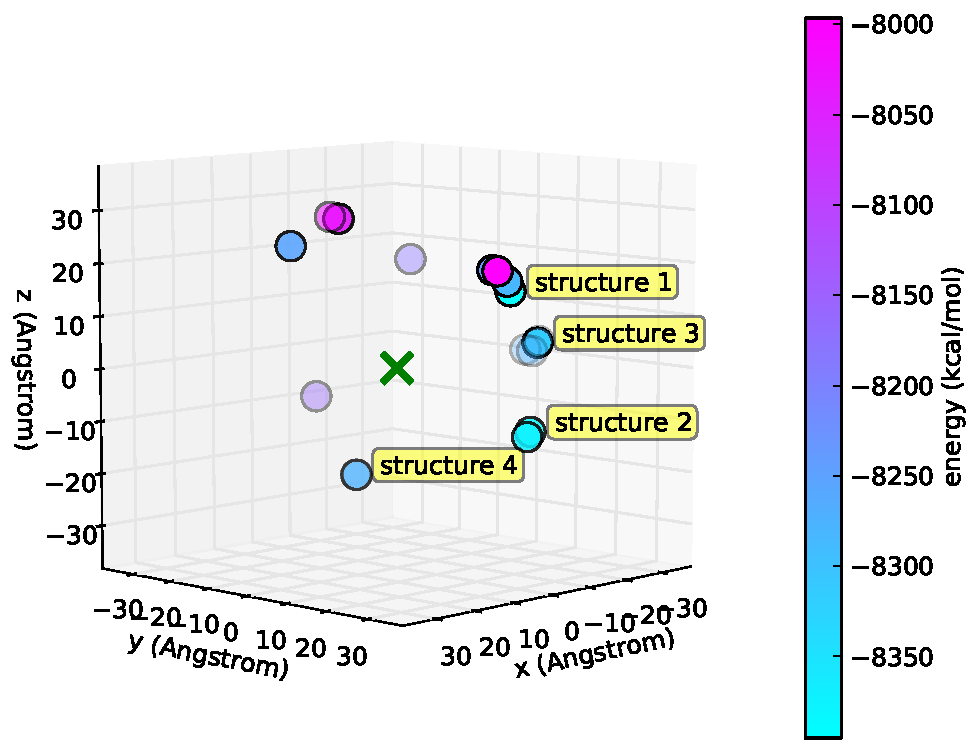
\includegraphics[width=1.0\textwidth]{figures/GMIN/CitA_phi_theta_3D.pdf}
%        \end{figure}     
%
%    \end{columns}  

        \begin{figure}
            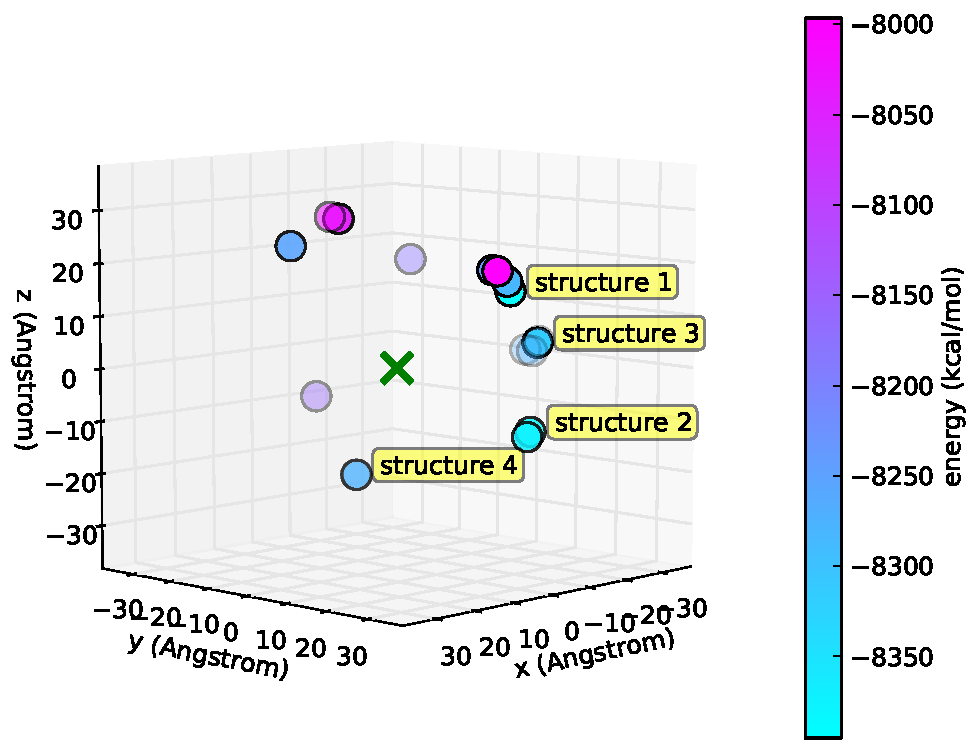
\includegraphics[width=0.8\textwidth]{figures/GMIN/CitA_phi_theta_3D.pdf}
        \end{figure}      


\end{frame}     


% ============================================================================ %

\begin{frame}
    \frametitle{Results}
    \framesubtitle{GMIN Basin Hopping} 

    \vspace{0.06\topmargin}

    \begin{columns}[t]
        \column{.5\linewidth}
        1)
        \vspace{-4ex}
        \begin{figure}
            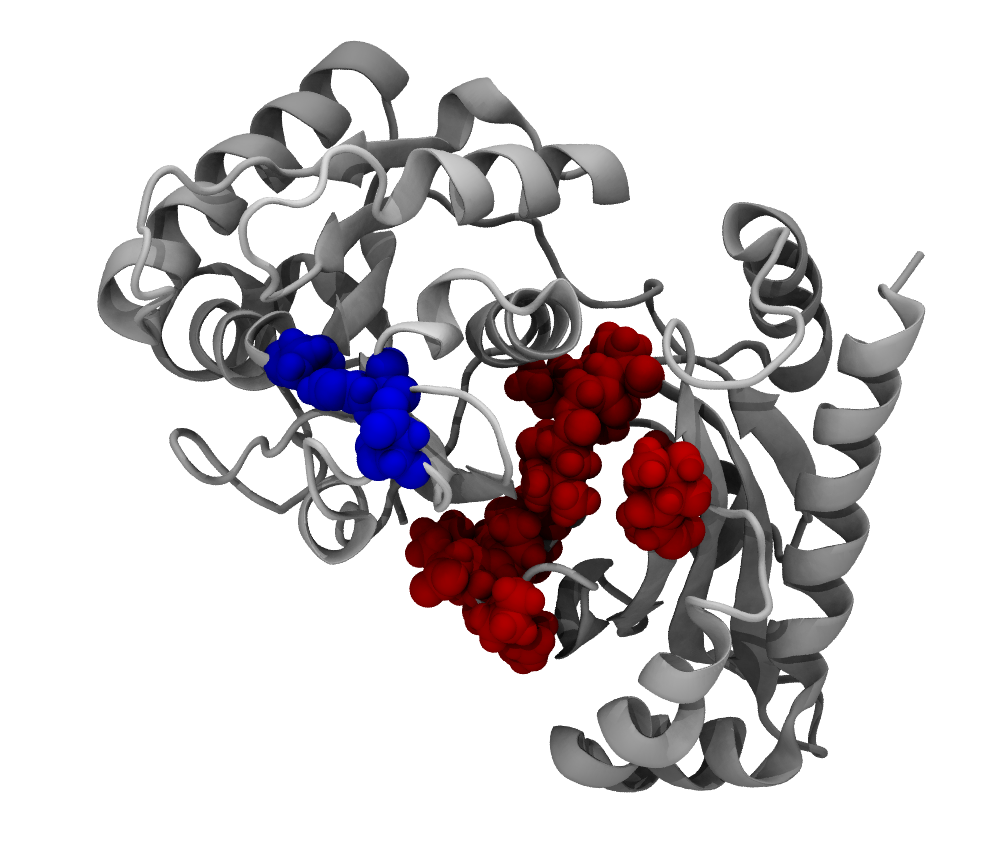
\includegraphics[width=0.85\textwidth]{figures/Complex_structures/structure1.png}  
        \end{figure}      
        3)
        \vspace{-8ex}
        \begin{figure}
            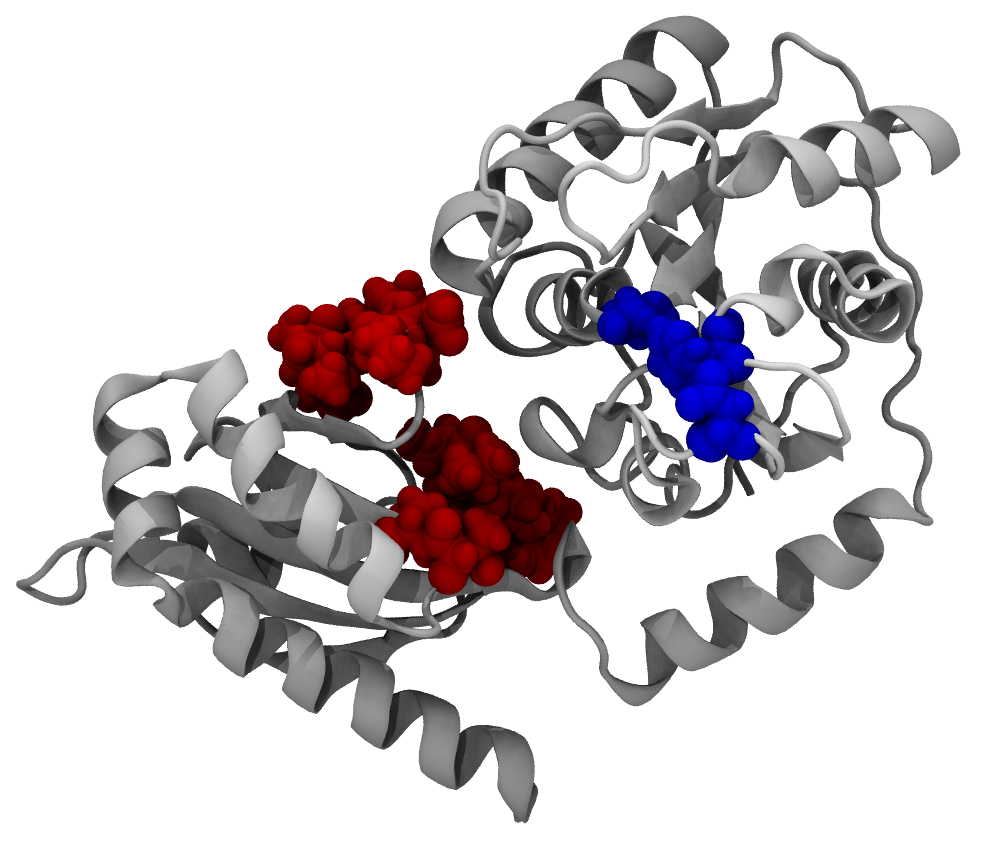
\includegraphics[width=0.85\textwidth]{figures/Complex_structures/structure3.png}   
        \end{figure}       

        \column{.5\linewidth}
        2)
        \vspace{-4ex}
        \begin{figure}
            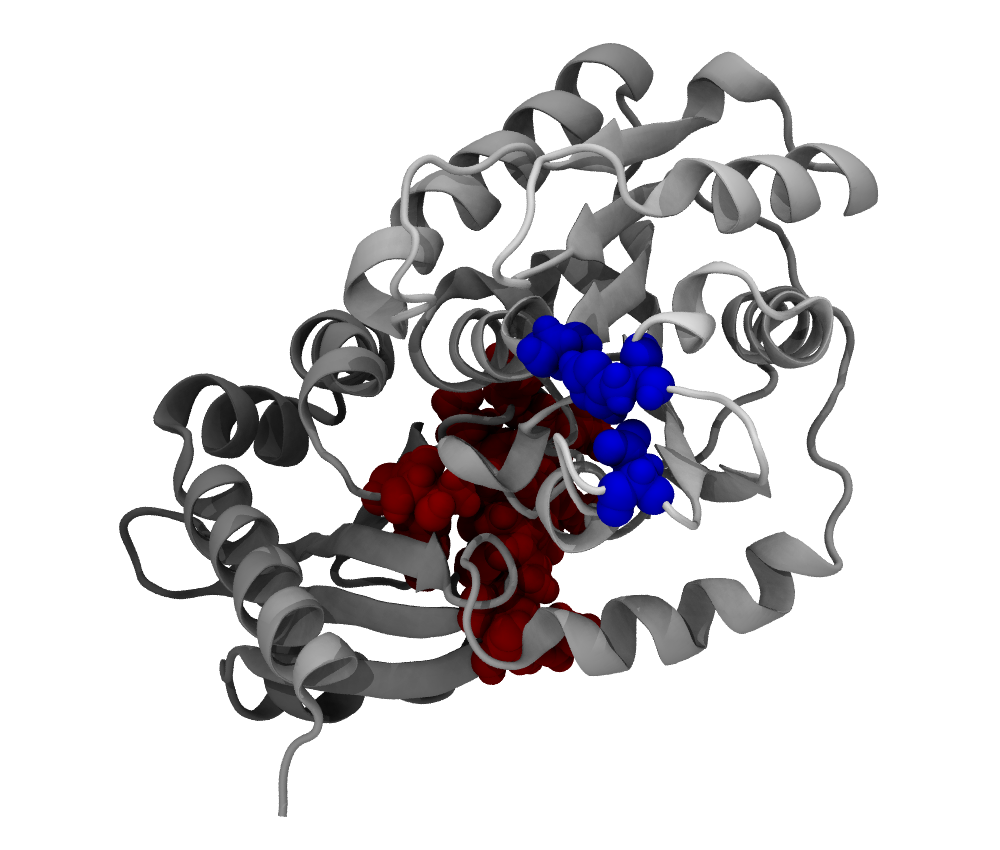
\includegraphics[width=0.85\textwidth]{figures/Complex_structures/structure2.png}  
        \end{figure}      
        4)
        \vspace{-8ex}
        \begin{figure}
            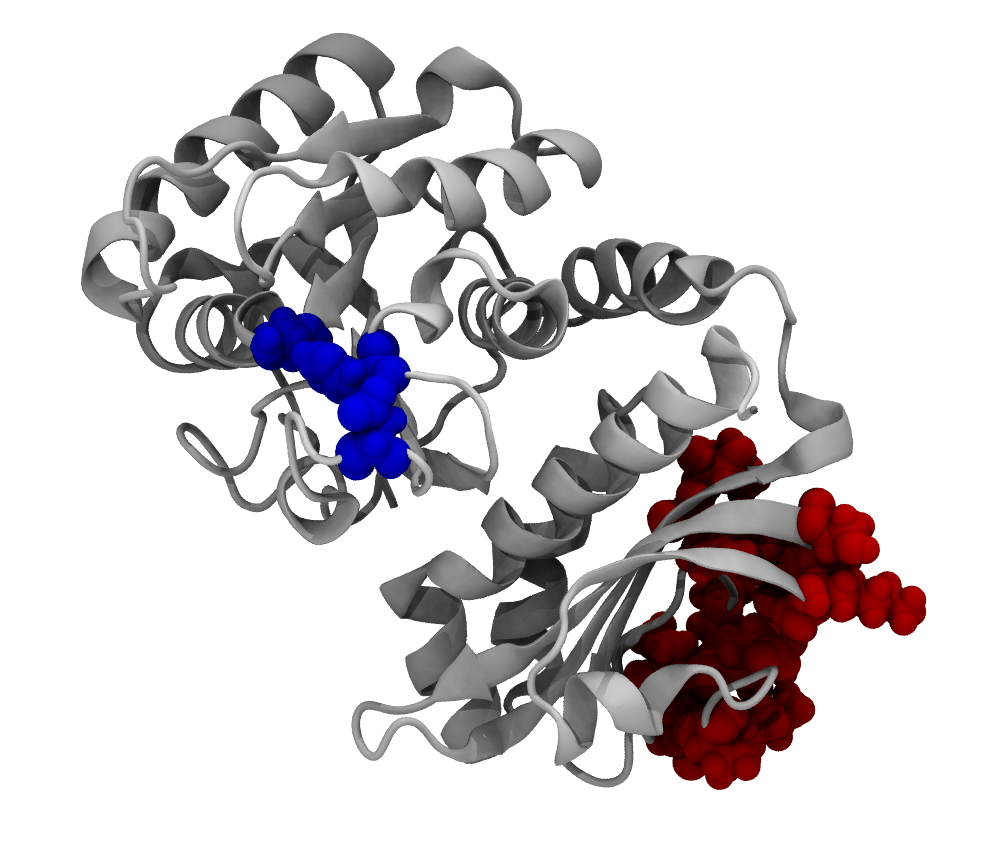
\includegraphics[width=0.85\textwidth]{figures/Complex_structures/structure4.png}   
        \end{figure}       

    \end{columns}  


\end{frame}      

% ============================================================================ %

\begin{frame}
    \frametitle{Results}
    \framesubtitle{Fusion Protein MD -- Secondary Structure}  

    \centering
    Secondary Structure is stable during 100 ns \\
    (Supplementary Material)
%    \begin{figure}
%        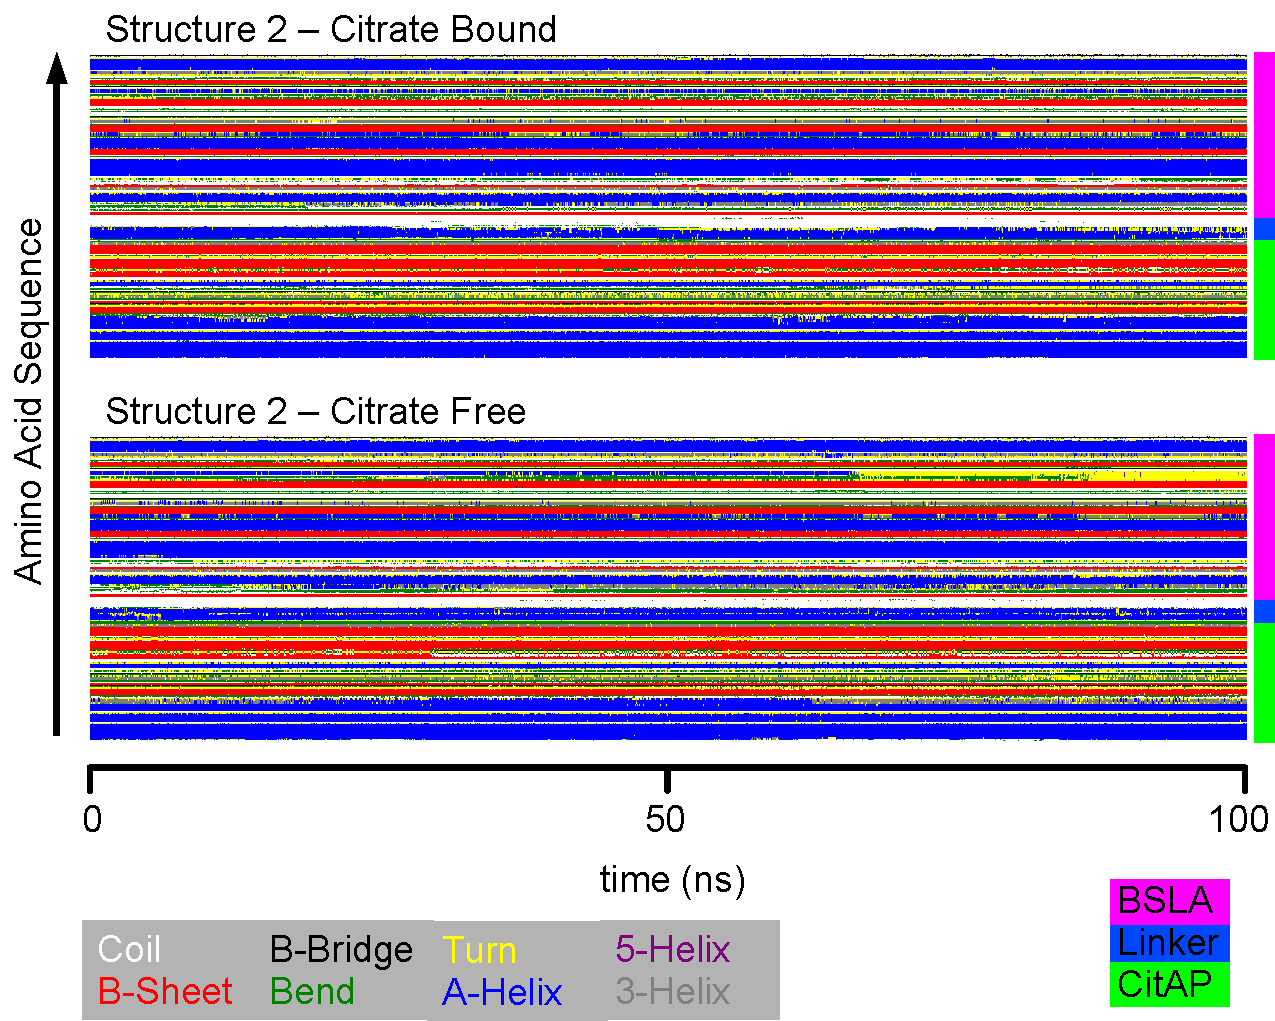
\includegraphics[width=0.78\textwidth]{figures/DSSP/dssp_presentation.pdf}
%    \end{figure}        
    
\end{frame}      


% ============================================================================ %

\begin{frame}
    \frametitle{Results}
    \framesubtitle{Fusion Protein MD -- Hydrophobic Contacts}  

    \vspace{0.06\topmargin}

    \begin{figure}
        \begin{minipage}[]{0.45\linewidth}
            \centering
            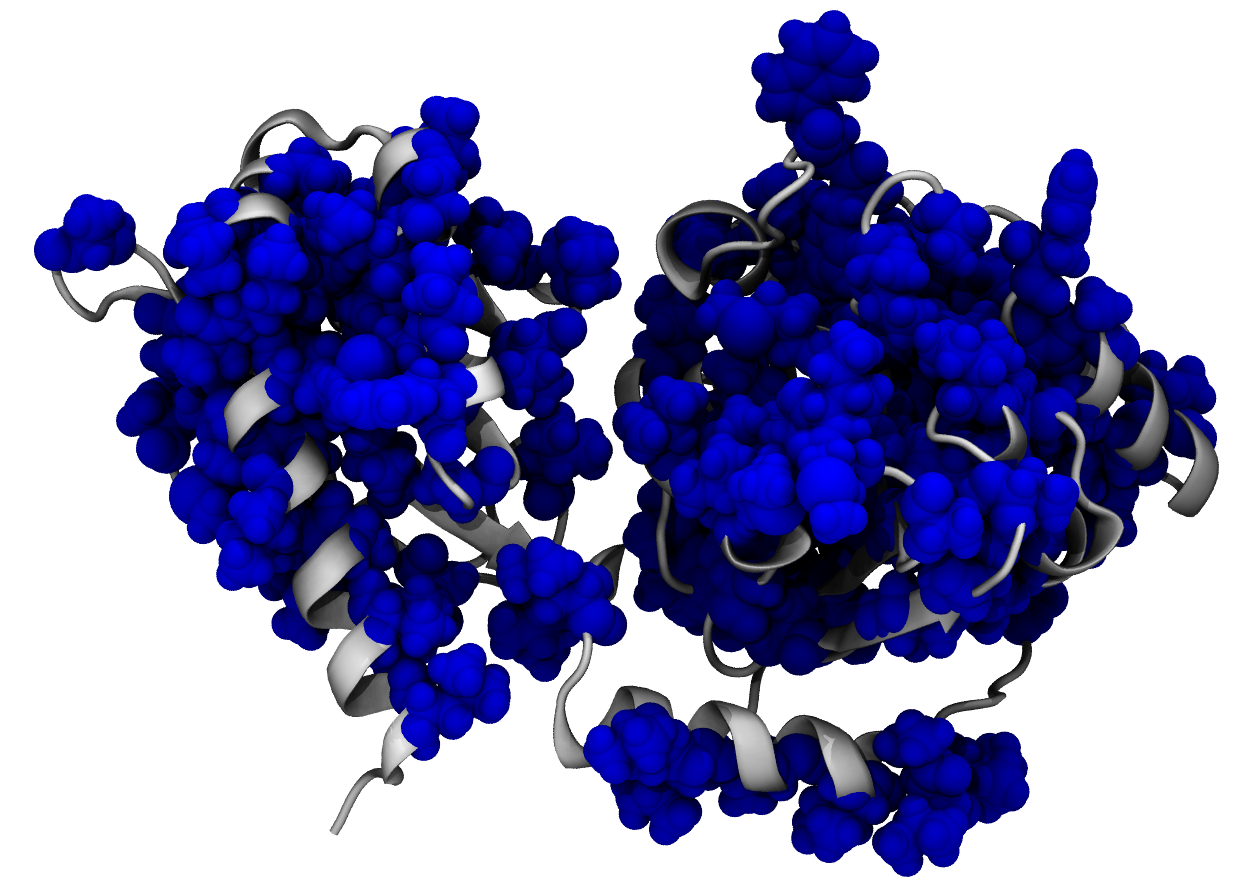
\includegraphics[width=\textwidth]{figures/Complex_hydrophobic_core/hydrophobic_core_linker.png}
        \end{minipage}
    \hspace{0.5cm}
        \begin{minipage}[]{0.45\linewidth}
            \centering
            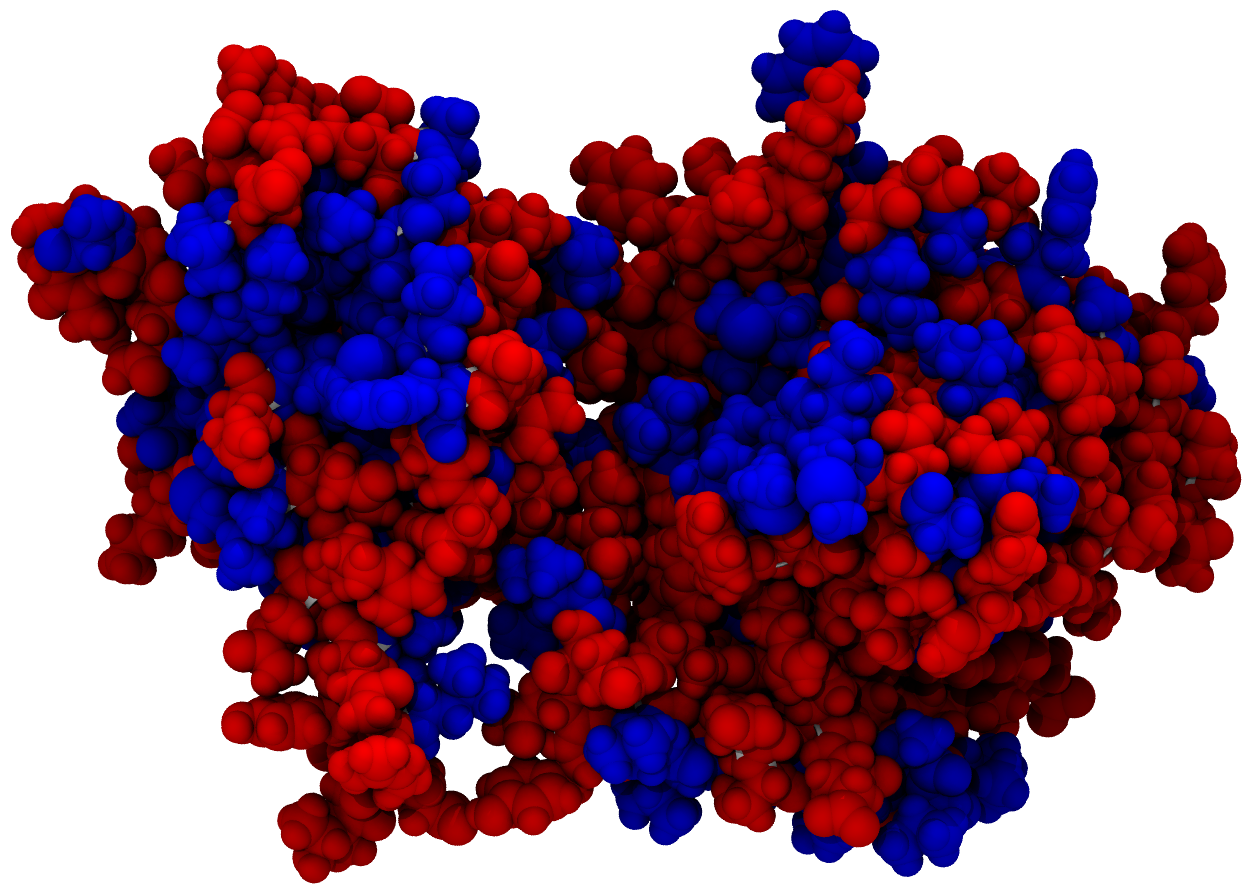
\includegraphics[width=\textwidth]{figures/Complex_hydrophobic_core/protein.png}
        \end{minipage}
    \end{figure}     
 
    
\end{frame}       
 
% ============================================================================ %

\begin{frame}
    \frametitle{Results}
\framesubtitle{Fusion Protein MD}% -- Trajectory}  

    \vspace{0.94\topmargin}

    \begin{figure}
        \hspace{0.0\textwidth}
        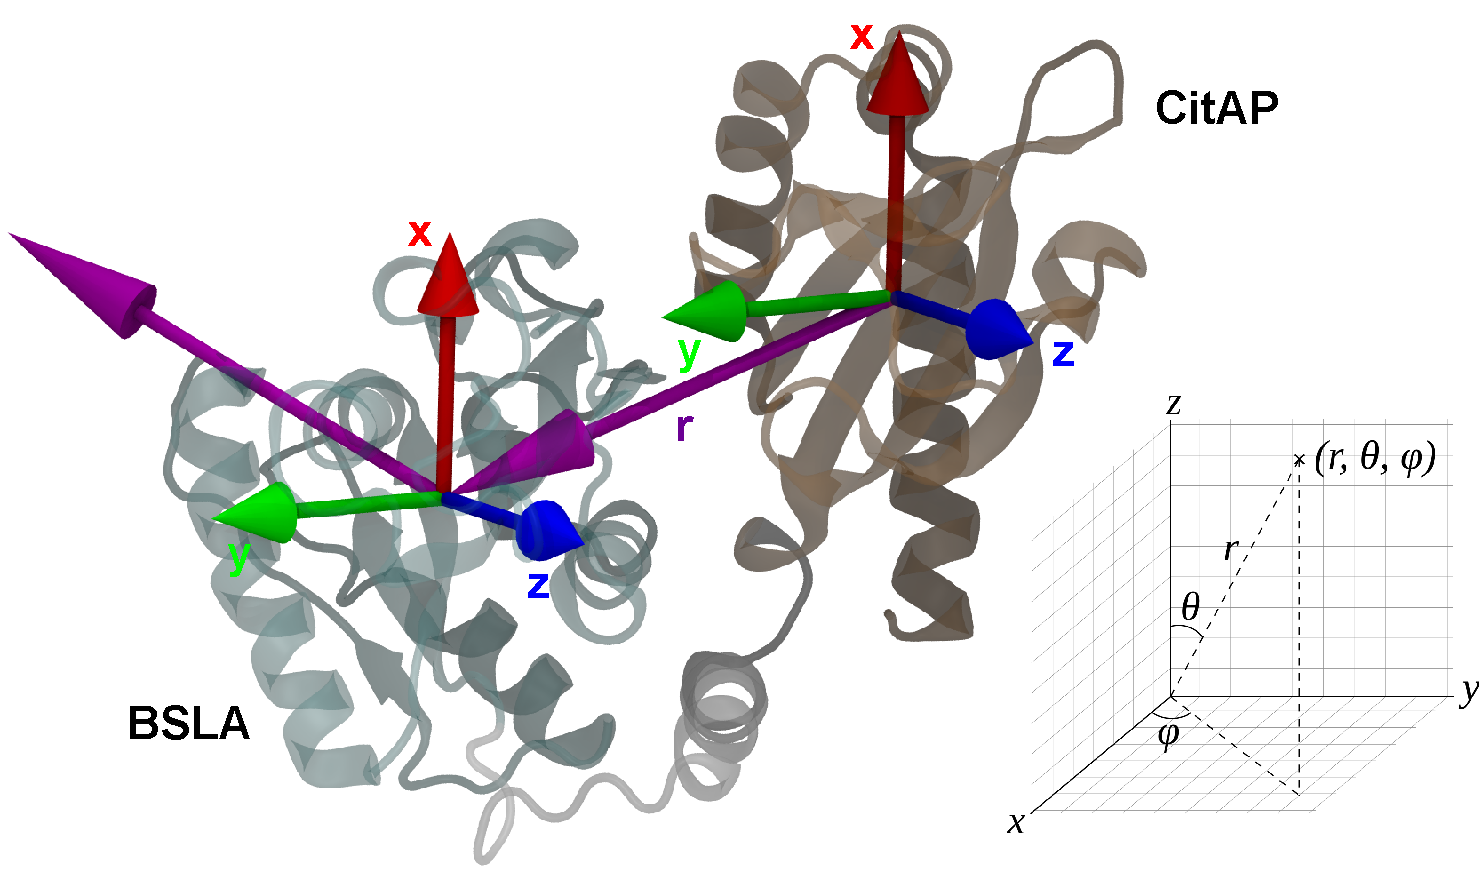
\includegraphics[width=0.40\textwidth]{figures/Collective_coords/collective_coords.pdf}
    \end{figure}     

    \vspace{-0.5cm}
 
%    \vspace{0.06\topmargin}

    \begin{columns}[t]
        \column{.5\linewidth}
        \vspace{-4ex}
        \begin{figure}
            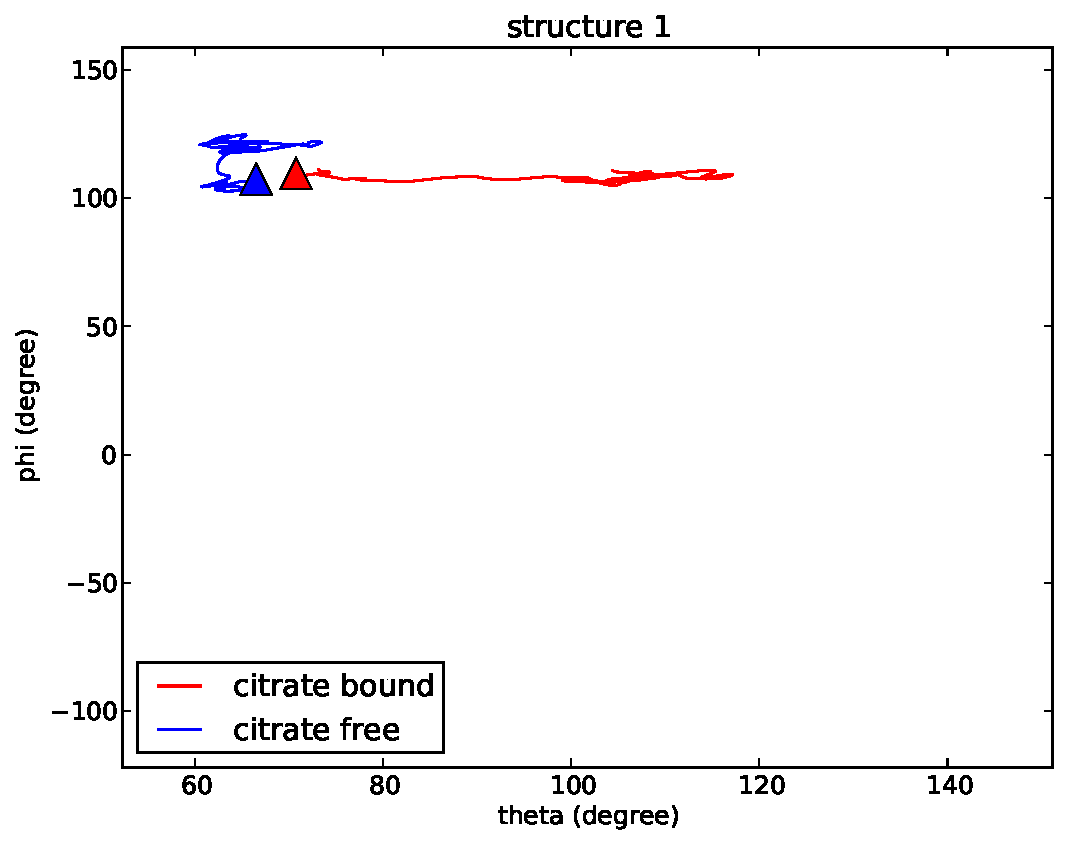
\includegraphics[width=0.85\textwidth]{figures/Complex_trajectory/collecitve_coords_structure1.pdf}  
        \end{figure}      
        \vspace{-5ex}
        \begin{figure}
            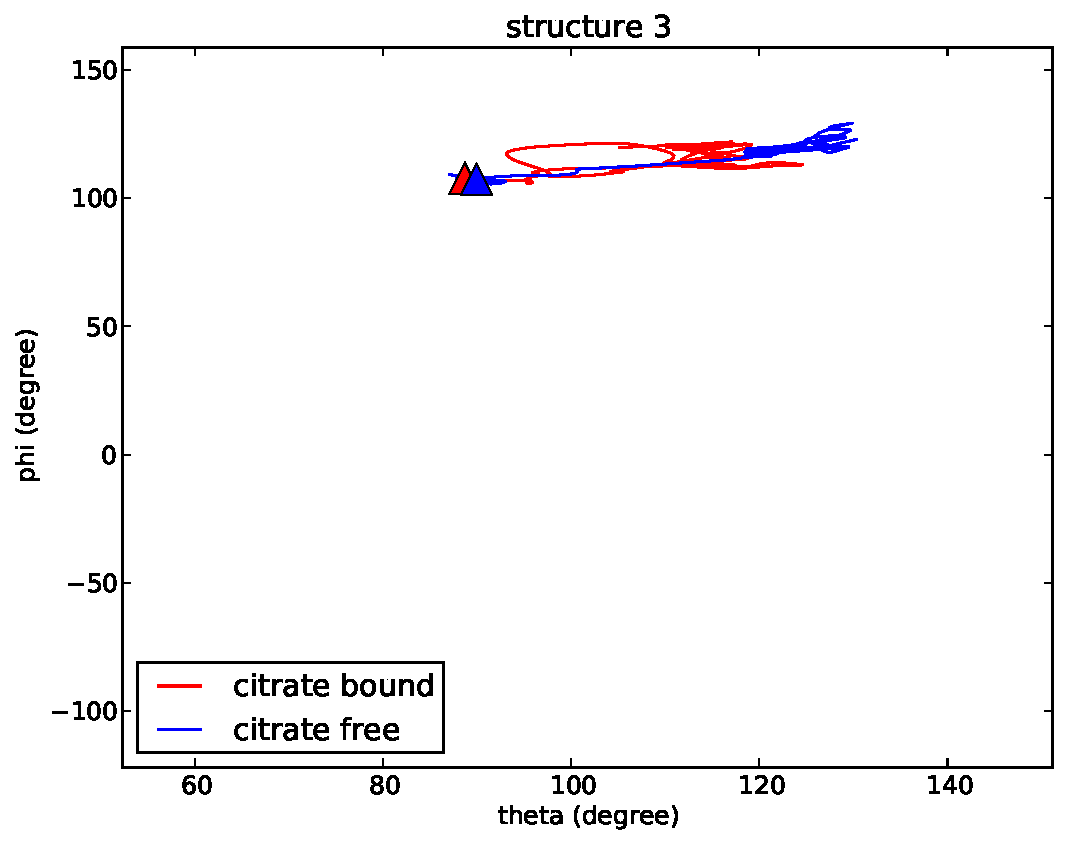
\includegraphics[width=0.85\textwidth]{figures/Complex_trajectory/collecitve_coords_structure3.pdf}  
        \end{figure}       

        \column{.5\linewidth}
        \vspace{-4ex}
        \begin{figure}
            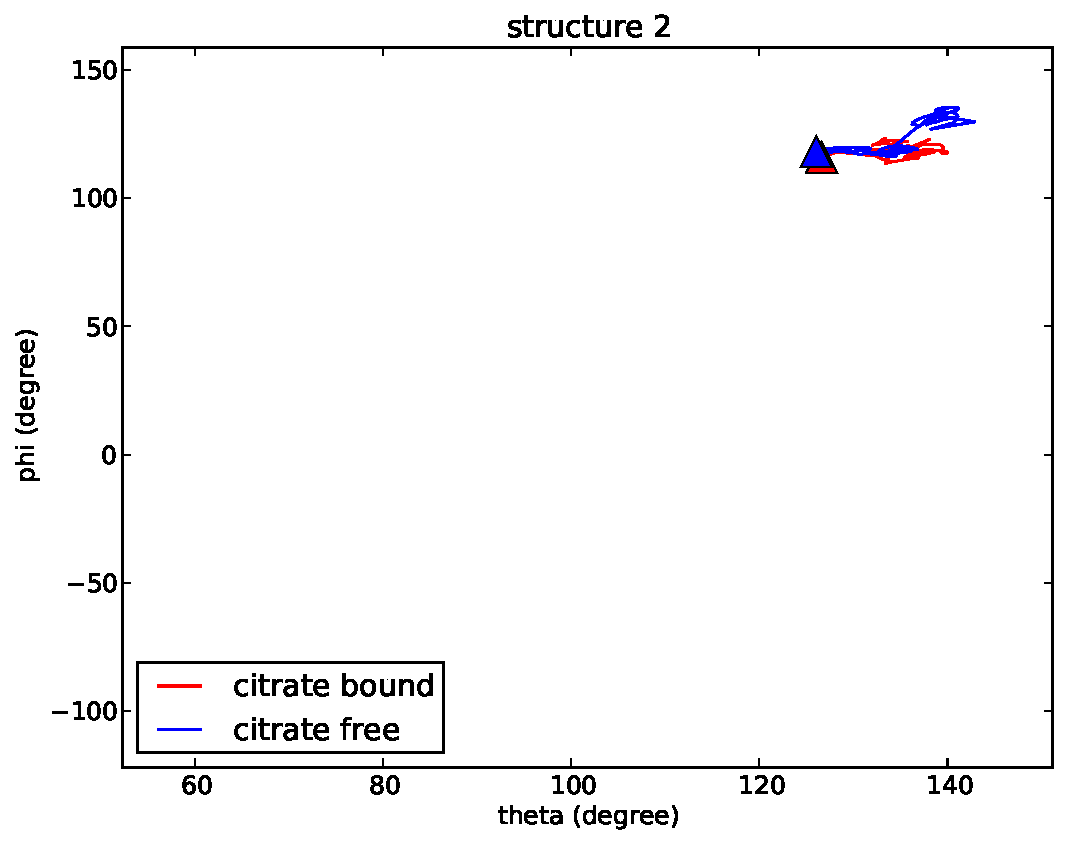
\includegraphics[width=0.85\textwidth]{figures/Complex_trajectory/collecitve_coords_structure2.pdf}  
        \end{figure}      
        \vspace{-5ex}
        \begin{figure}
            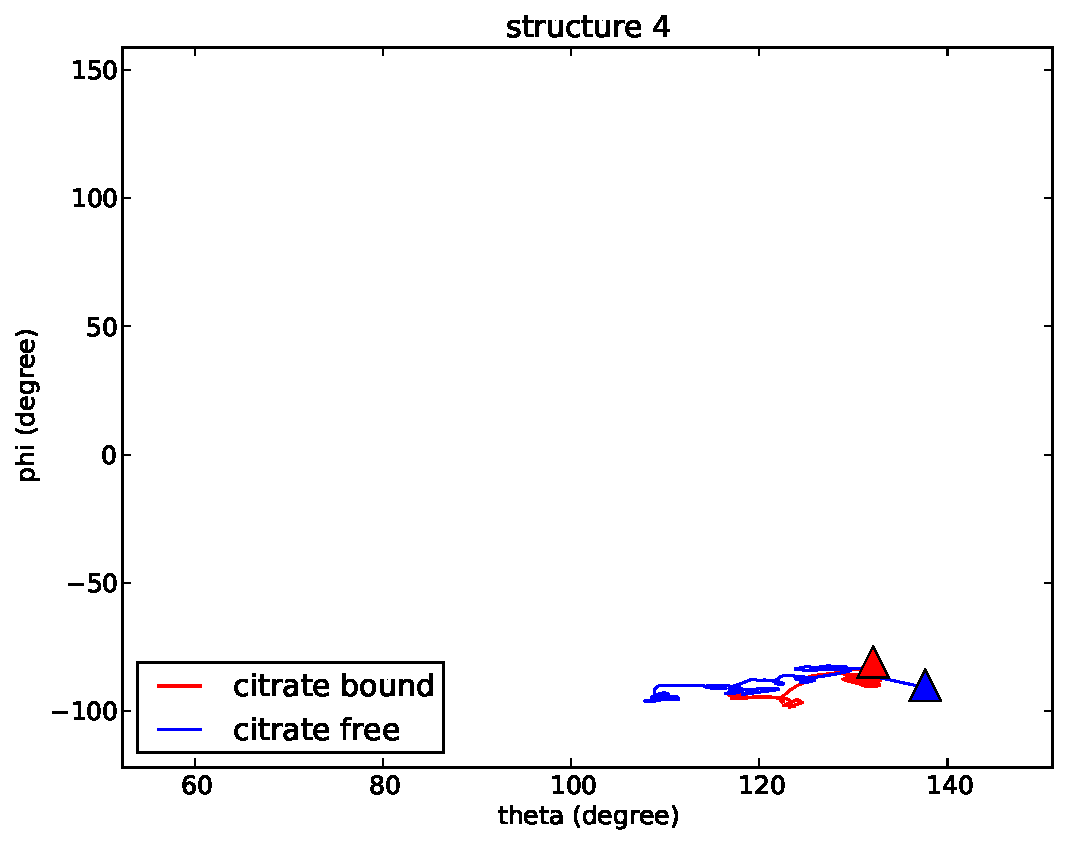
\includegraphics[width=0.85\textwidth]{figures/Complex_trajectory/collecitve_coords_structure4.pdf}   
        \end{figure}       

    \end{columns}   
    
\end{frame}        

% ============================================================================ %

\begin{frame}
    \frametitle{Results}
    \framesubtitle{Fusion Protein MD -- TYR/TRP Fluorescence}  

%    \vfill
    \vspace{-4ex}

    \begin{columns}[t]
        \column{.5\linewidth}
        \begin{figure}
            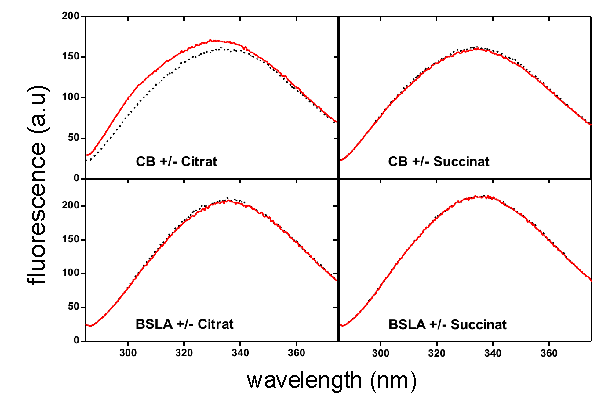
\includegraphics[width=1.0\textwidth]{figures/TyrTrp/TyrTrp_experiment.pdf}
        \end{figure}         

        \centering
        Excitation: 278 nm 

        \begin{center}
        \begin{table}
        \tiny
        \begin{tabular}{l c c} 
                       & Absorbtion & Fluorescence \\
            \hline
            Tyrosine   & 280 nm & 348 nm \\
            Tryptophan & 274 nm & 303 nm \\
        \end{tabular}
        \end{table}
        \end{center}

        \column{.5\linewidth}
        \begin{figure}
            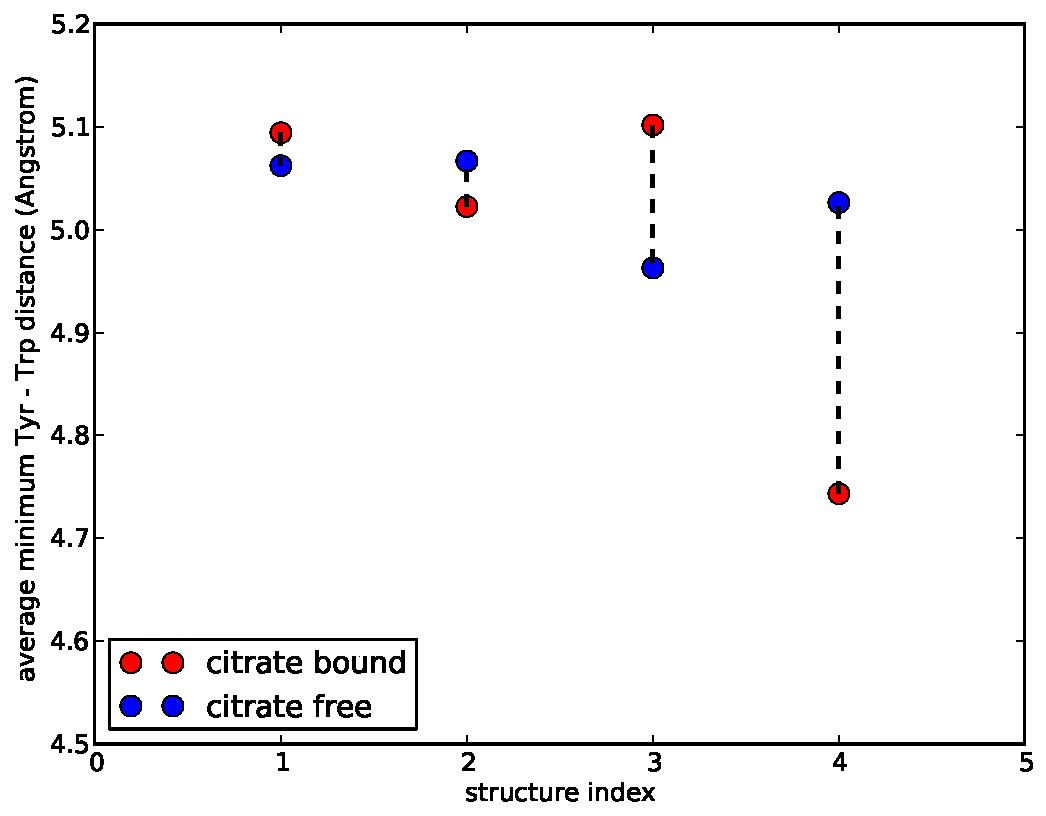
\includegraphics[width=1.0\textwidth]{figures/TyrTrp/average_mindist_TyrTrp.pdf}
        \end{figure}      

        \centering
        Tryptophan only in BSLA

    \end{columns}    

    \vfill

    \vspace{2ex}
    \tiny
    \fullcite{FluorescenceWeb}
 
\end{frame}        

% ============================================================================ %

\begin{frame}
    \frametitle{Results}
    %\framesubtitle{Fusion Protein MD -- Active Site Distances}  
    \framesubtitle{Fusion Protein MD}  

    \vspace{0.94\topmargin}

    \begin{figure}
        \hspace{0.1\textwidth}
        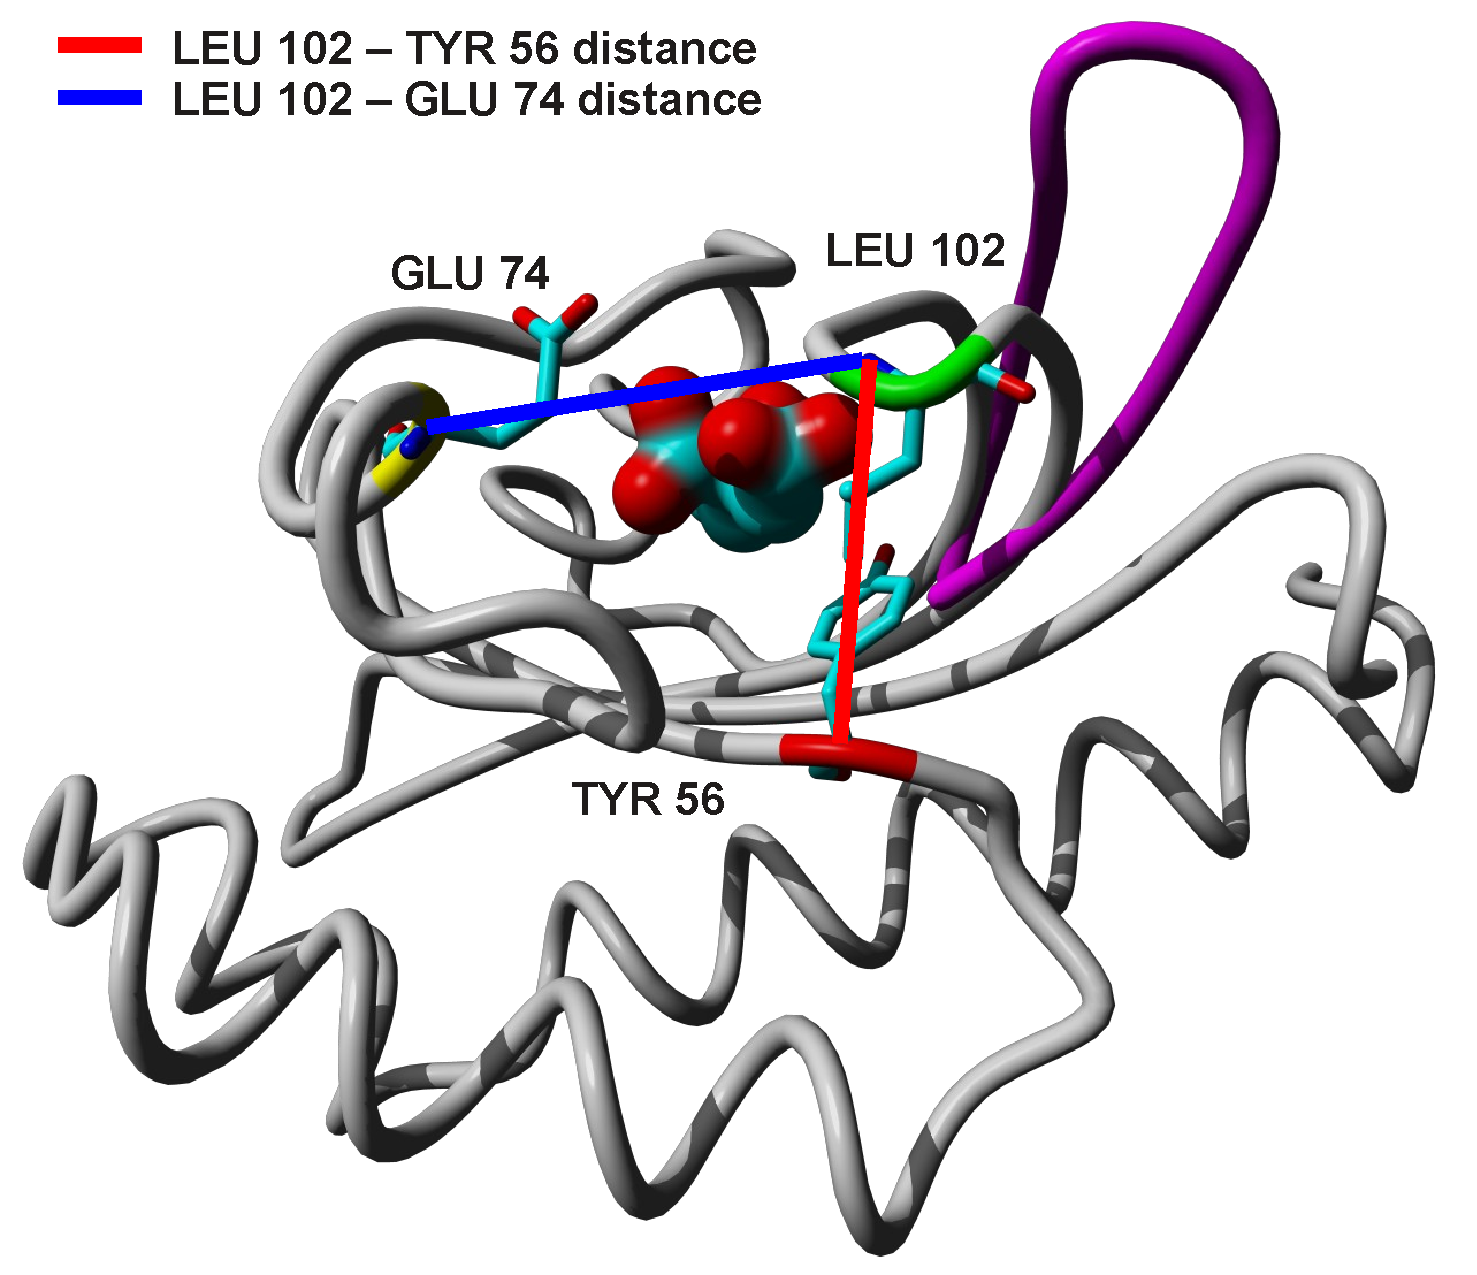
\includegraphics[width=.3\linewidth]{figures/CitA_pocket2.pdf}
        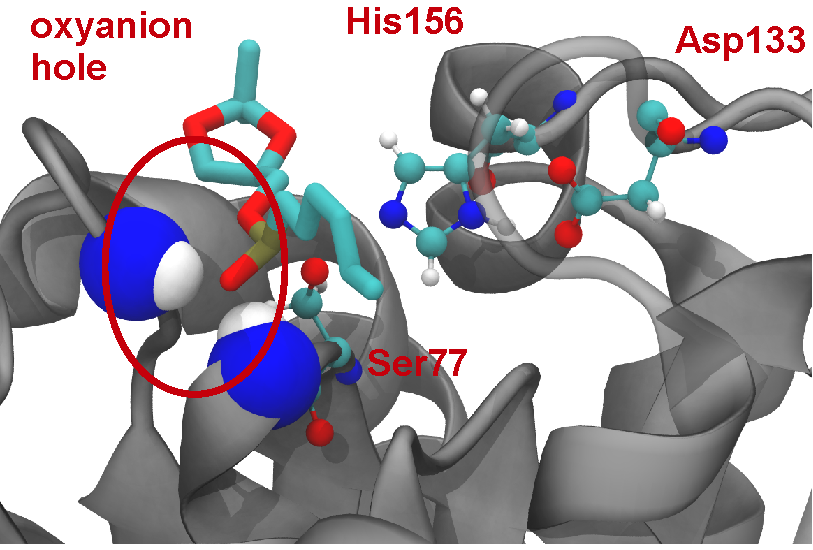
\includegraphics[width=.3\textwidth]{figures/BSLA_pocket/BSLA_pocket_cartoon.pdf}
    \end{figure}     

    \vspace{-0.5cm} 

    \vfill

    \begin{columns}[]
        \column{.5\linewidth}
        \vfill
        \centering
        Open / Closed Conformation
        \begin{figure}
            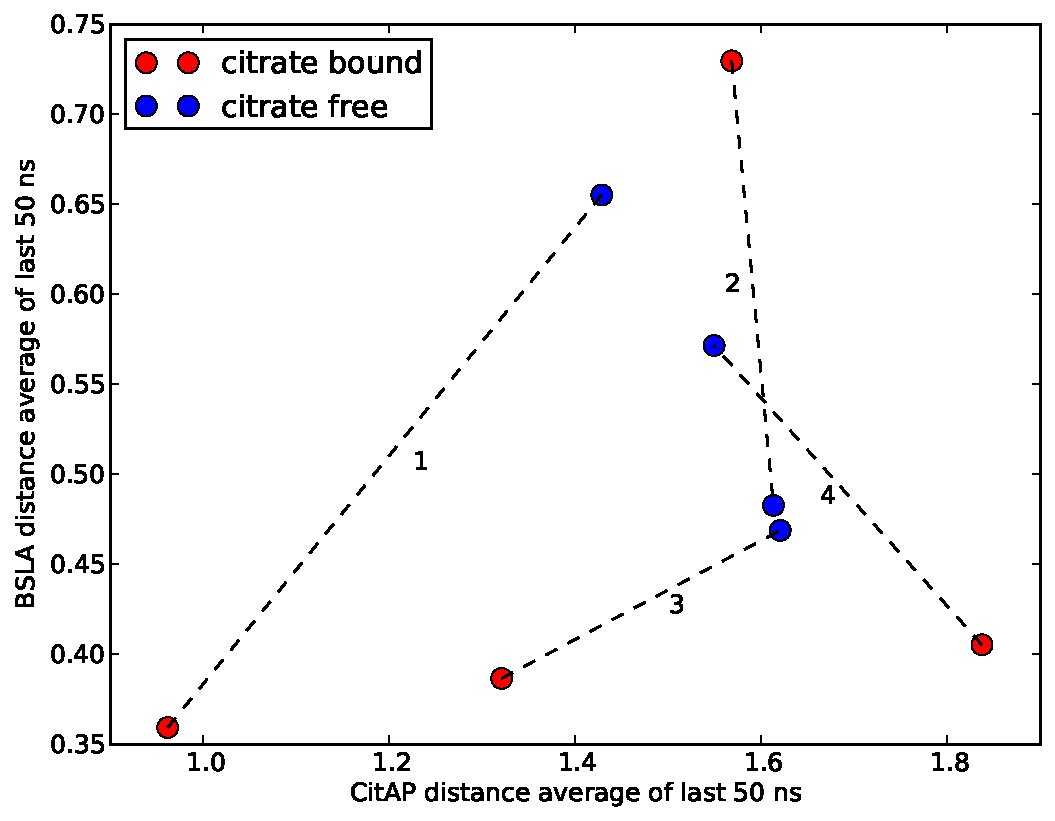
\includegraphics[width=\textwidth]{figures/CitAP_BSLA_distance/BSLA_CitAP_analyzed_with_average_of_last_50_ns.pdf}  
        \end{figure}         

        \column{.5\linewidth}
        \vfill
        \centering
        Flexibility
        \begin{figure}
            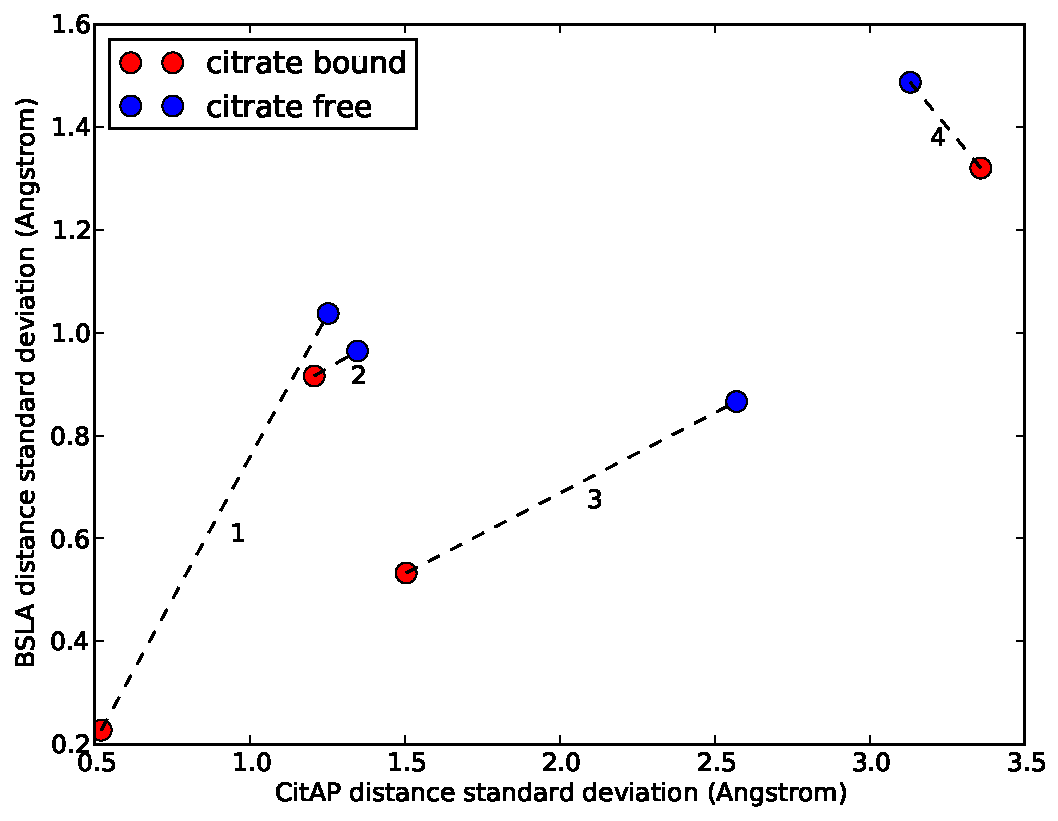
\includegraphics[width=\textwidth]{figures/CitAP_BSLA_distance/BSLA_CitAP_analyzed_with_standard_deviation.pdf}  
        \end{figure}      

    \end{columns}    

    \vfill 

\end{frame}        
 
% ============================================================================ %

\section{Conclusions}

\begin{frame}
    \frametitle{Conclusions}

    \begin{itemize}
        \item<1-> Solo MD simulations gave expected results
        \item<2-> 4 different fusion protein structures
        \item<3-> Secondary structure is stable
        \item<4-> 2 hydrophobic cores
        \item<5-> Systems not equilibrated after 100 ns
        \item<6-> Only structure 4 in accordance with TYR/TRP fluorescence
        \item<7-> Binding pocket dynamics different in fusion protein (more flexible)
        \item<8-> No unique active site distance correlation between domains
    \end{itemize}

\end{frame}        

% ============================================================================ %

\section{Outlook}

\begin{frame}
    \frametitle{Outlook}

    \setstretch{2}

    \begin{itemize}
        \item<1-> Lack of experimental data
        \item<2-> Structural information required
            \begin{itemize}
                \item<2-> Full X-ray/NMR structure
                \item<2-> Information on global shape (SAXS)
                \item<2-> Intermolecular distances (FRET)
            \end{itemize}
        \item<3-> Coarse grained MD for equilibration (MARTINI force field)
    \end{itemize}

    \setstretch{1}

\end{frame}   

% ============================================================================ %

\begin{frame}
    \frametitle{Questions}

    \vfill
    \centering
    \Huge ?
    \vfill


\end{frame}   
 
% ============================================================================ %


\section{Supplementary Material}


\begin{frame}
    \frametitle{Methods}
    \framesubtitle{Forcefield: Amber99sb-ildn-nmr}

    Uncertainty weighted objective function: $\chi^2 = \sum_i(x_i^{Exp} - x_i)^2 / \sigma_i^2$

    \begin{figure}
        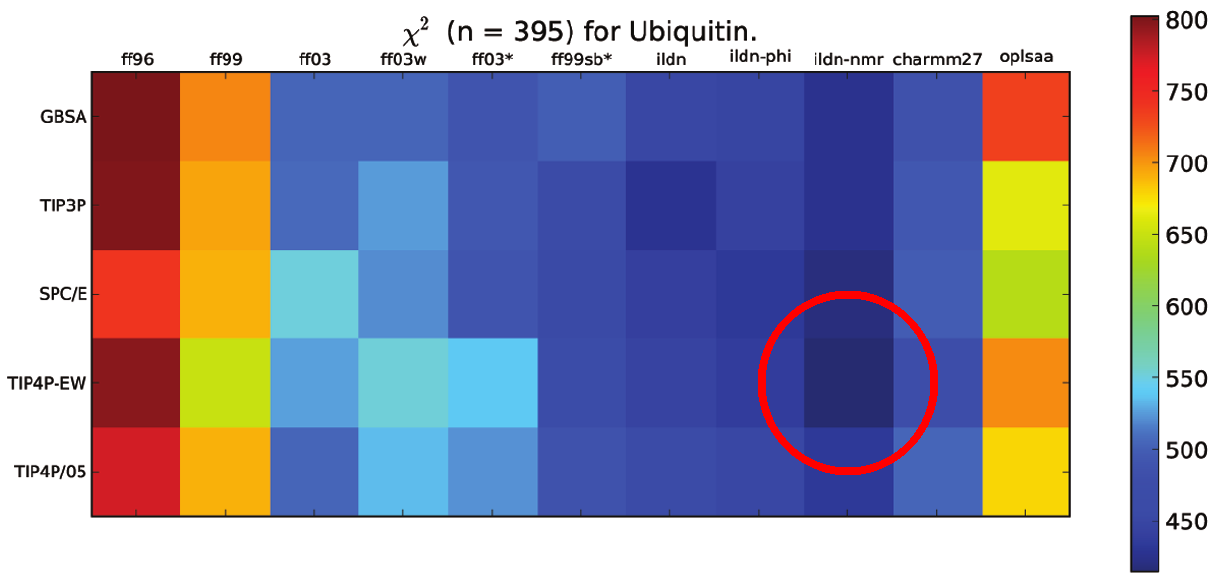
\includegraphics[width=\linewidth]{figures/forcefield_performance.png}
    \end{figure}        

    \tiny
    \fullcite{proteinFF}

%    K. A. Beauchamp, Y. Lin, R. Das and V. S. Pande,
%    \href{http://pubs.acs.org/doi/abs/10.1021/ct2007814}
%    {Are Protein Force Fields Getting Better?
%    A Systematic Benchmark on 524 Diverse NMR Measurements},
%    \textit{J. Chem. Theory Comput.},
%    8, 1409--1414, 2012
    

\end{frame}   

% ============================================================================ %

\begin{frame}
    \frametitle{Methods}
    \framesubtitle{Citrate Forcefield Parameterization}

    \begin{figure}
        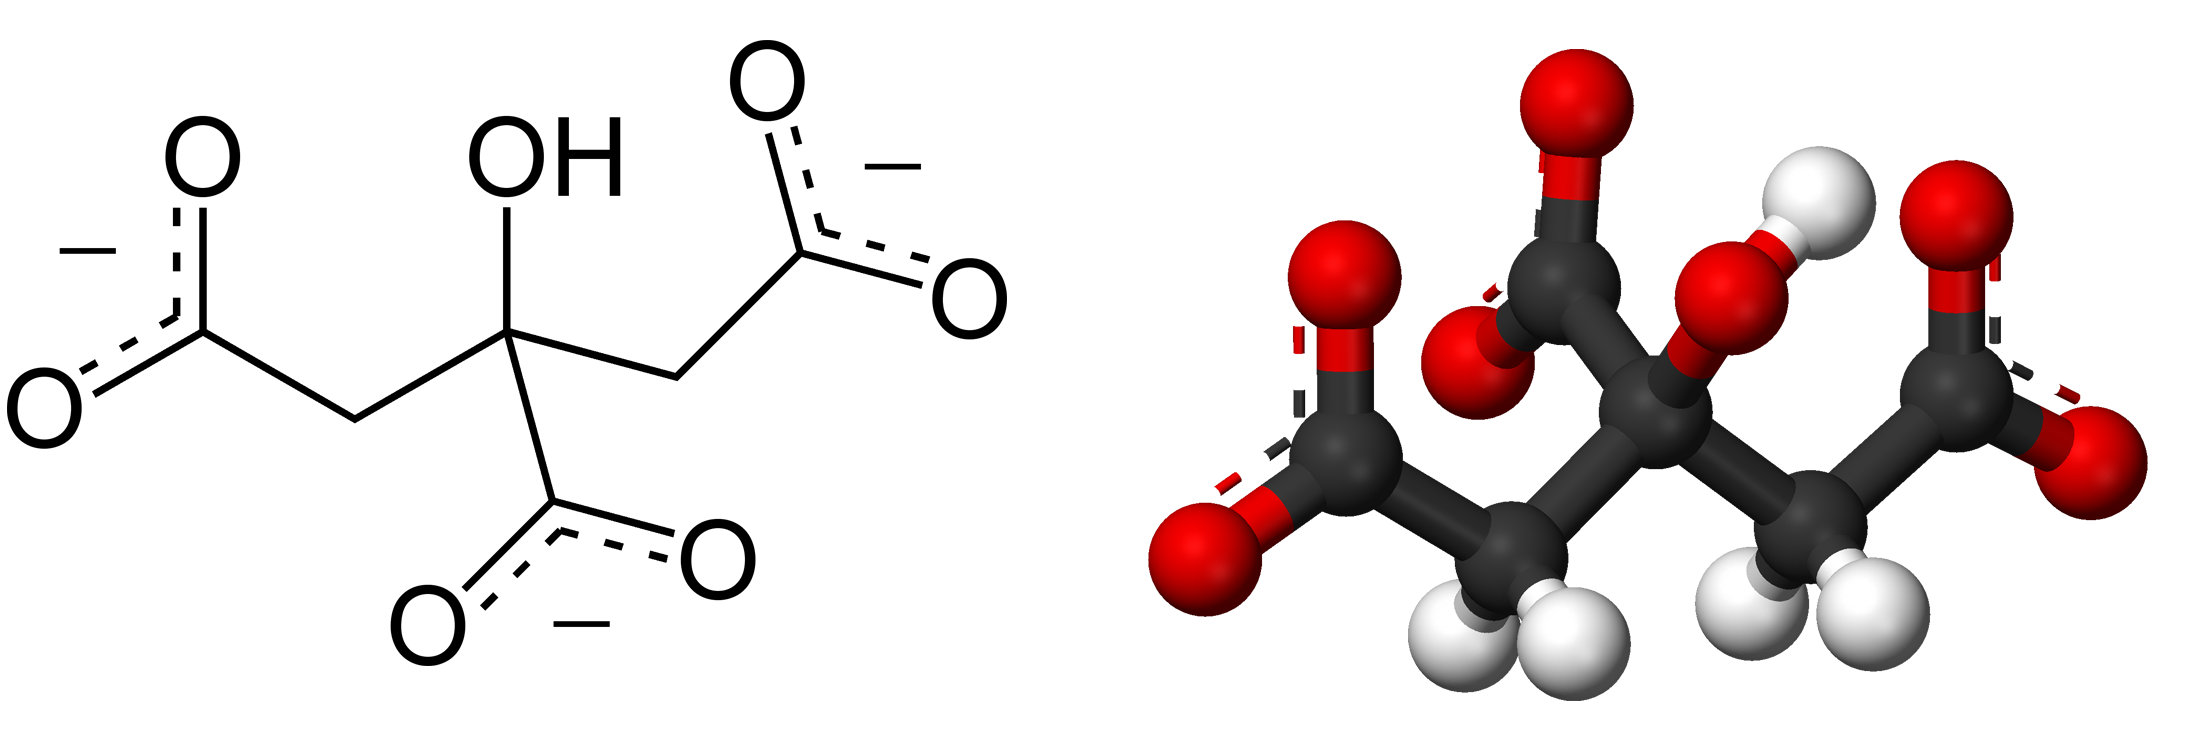
\includegraphics[width=.7\linewidth]{figures/citrate.png}
    \end{figure}      

    \begin{itemize}
        \item Parameterized with the general AMBER force field (GAFF) from Ambertools using ACPYPE
        \item Partial charges come from
        \begin{itemize}
            \item \textbf{Antechamber} -- AM1-BCC (parameterized fit to \textit{ab initio} calculations)
%            \item YASARA AutoSIMLES Server -- ''improved'' AM1-BCC
%            \item \textit{ab initio}
        \end{itemize}
    \end{itemize}

    \tiny
    \fullcite{ACPYPE}

\end{frame}   

% ============================================================================ %

\begin{frame}
    \frametitle{Results}
    \framesubtitle{Fusion Protein MD -- Secondary Structure}  

    \begin{figure}
        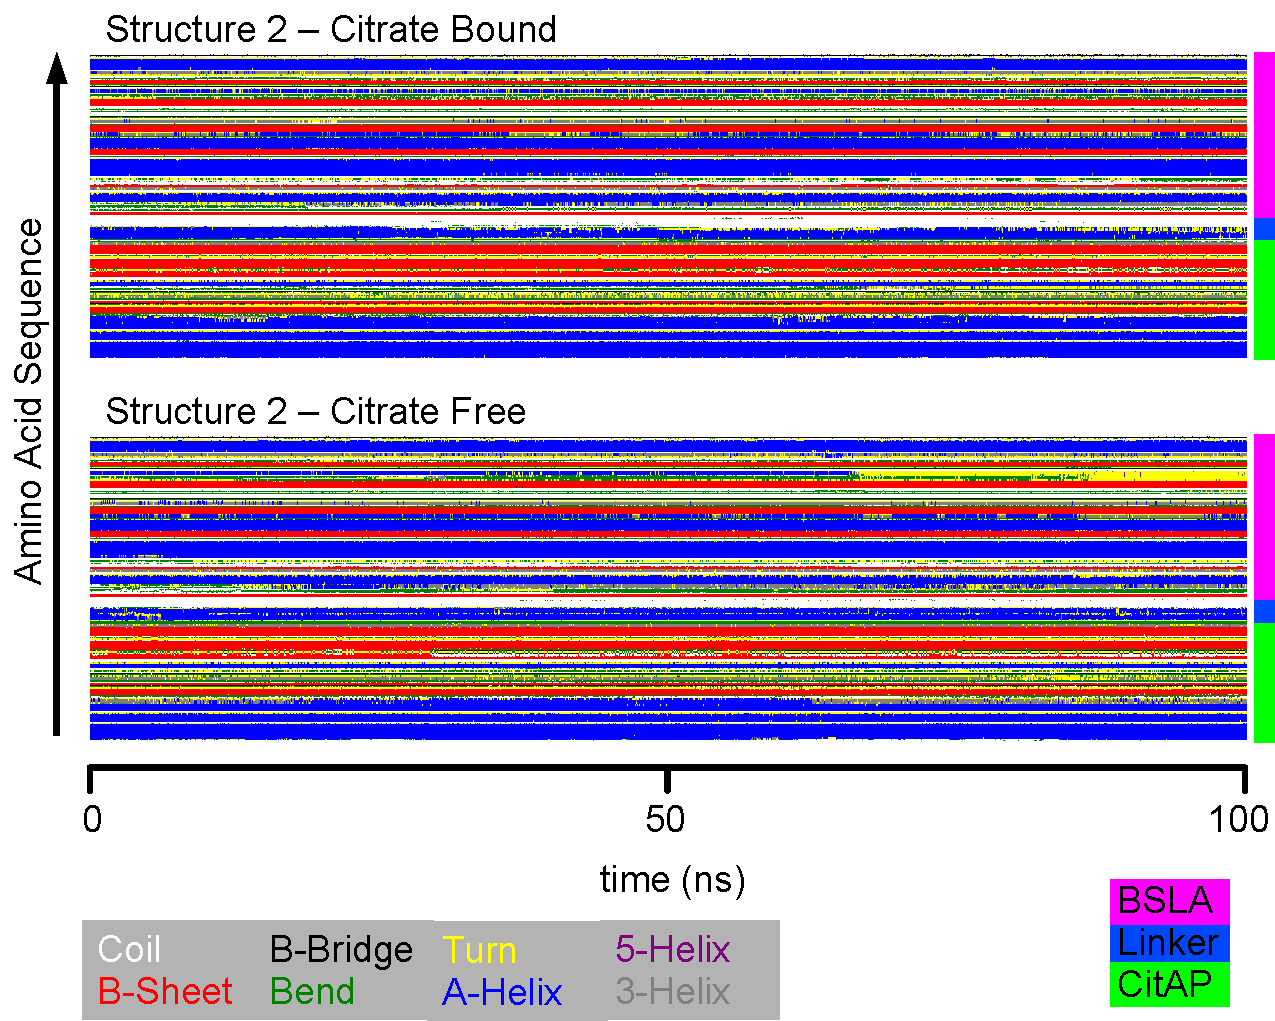
\includegraphics[width=0.78\textwidth]{figures/DSSP/dssp_presentation.pdf}
    \end{figure}        
    
\end{frame}      

% ============================================================================ %

\begin{frame}
    \frametitle{Results}
    \framesubtitle{Fusion Protein MD -- Favourable Contacts}  

    \vspace{0.06\topmargin}

    \begin{columns}[t]
        \column{.5\linewidth}
        \vspace{-4ex}
        \begin{figure}
            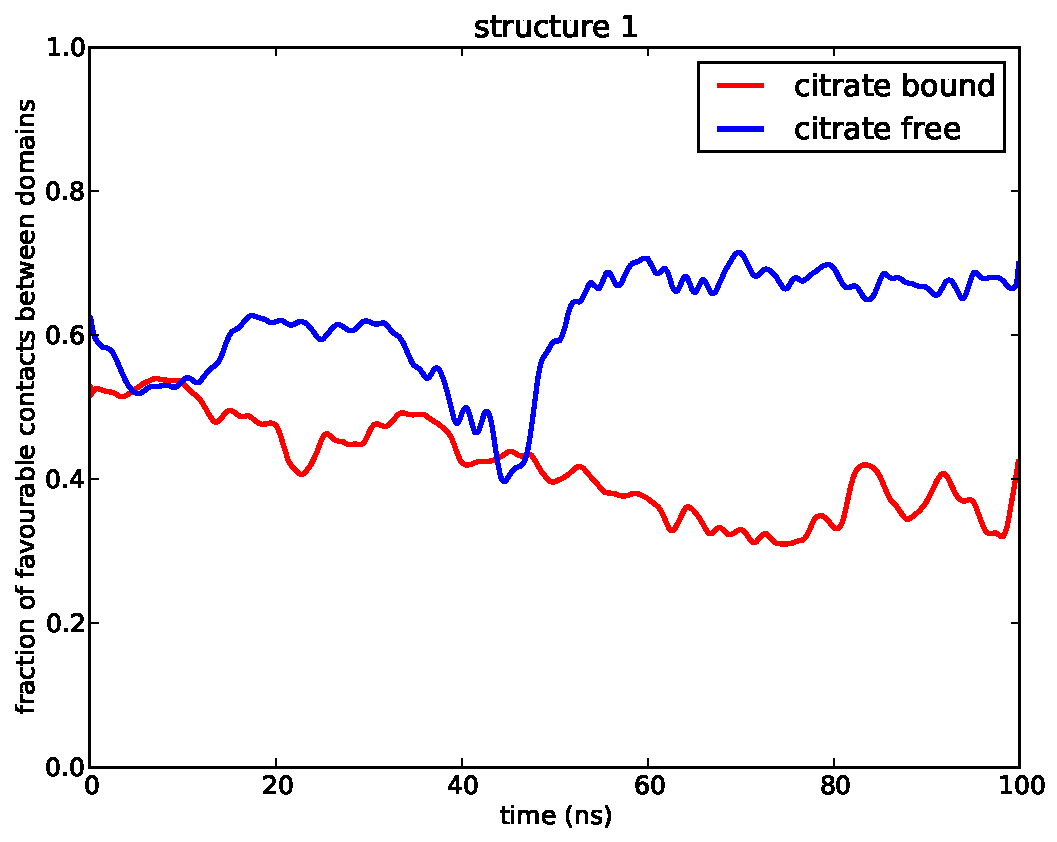
\includegraphics[width=0.85\textwidth]{figures/Complex_hydrophobic_core/favourable_cont_structure1.pdf}  
        \end{figure}      
        \vspace{-5ex}
        \begin{figure}
            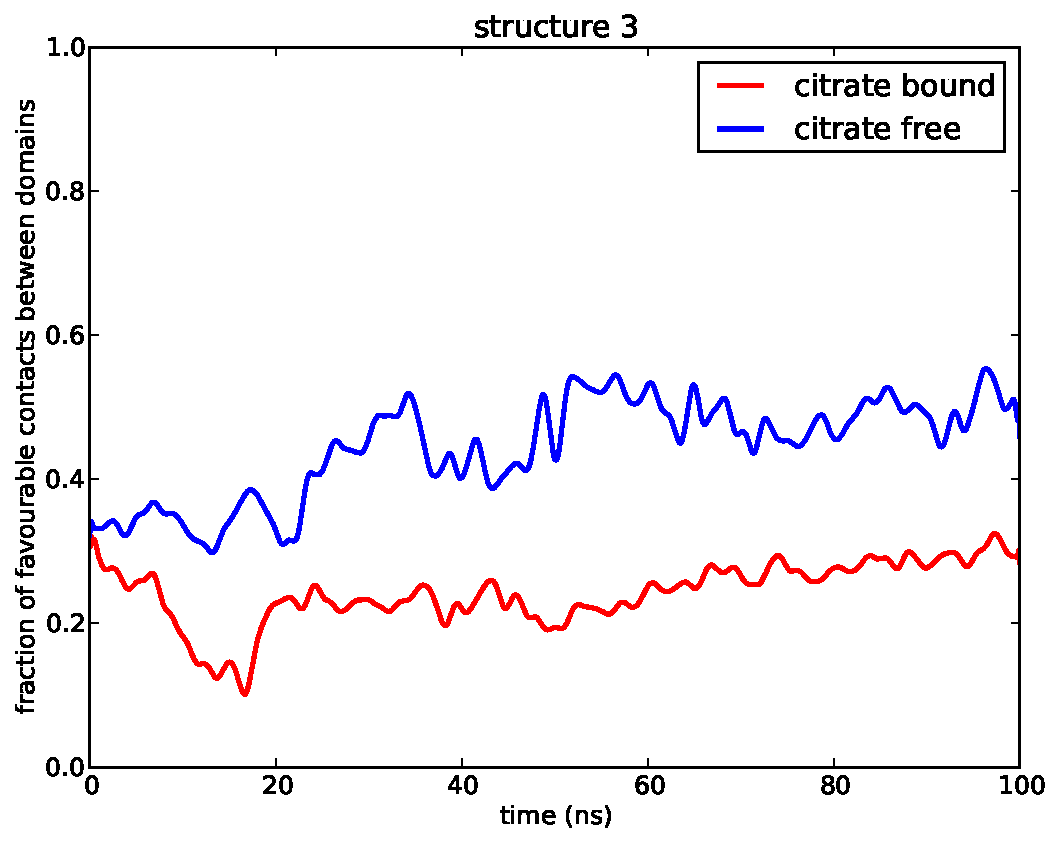
\includegraphics[width=0.85\textwidth]{figures/Complex_hydrophobic_core/favourable_cont_structure3.pdf}  
        \end{figure}       

        \column{.5\linewidth}
        \vspace{-4ex}
        \begin{figure}
            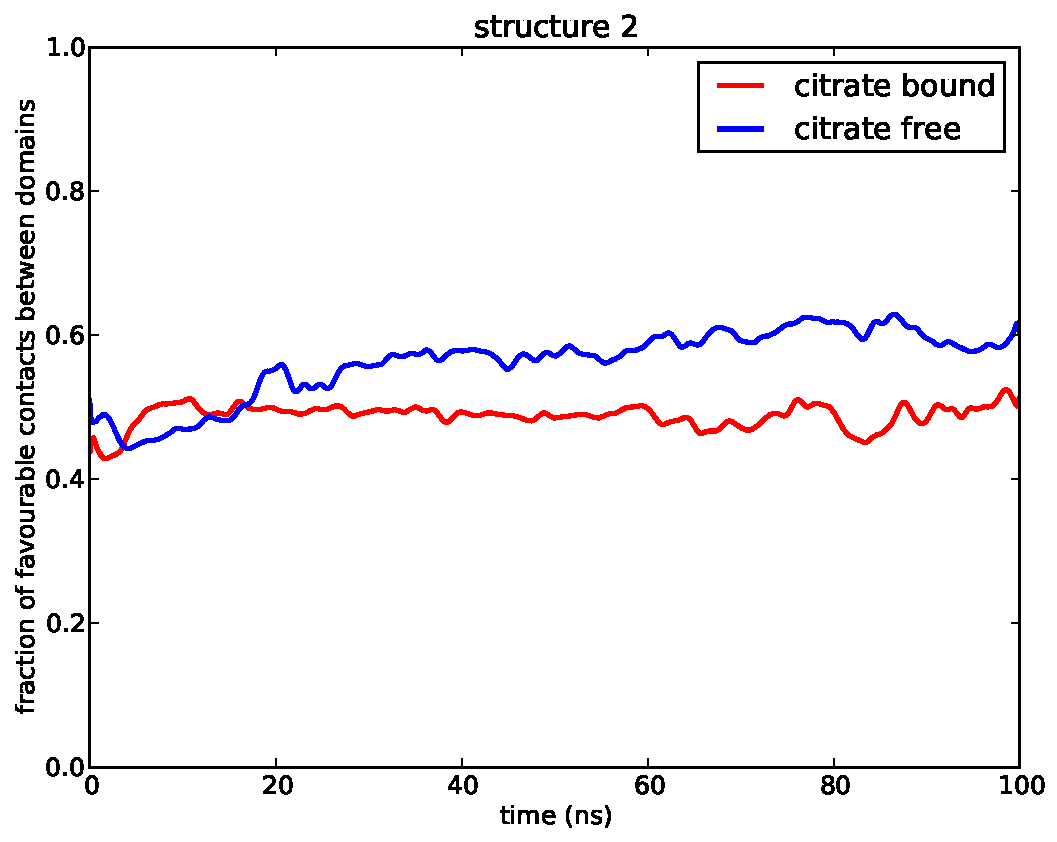
\includegraphics[width=0.85\textwidth]{figures/Complex_hydrophobic_core/favourable_cont_structure2.pdf}  
        \end{figure}      
        \vspace{-5ex}
        \begin{figure}
            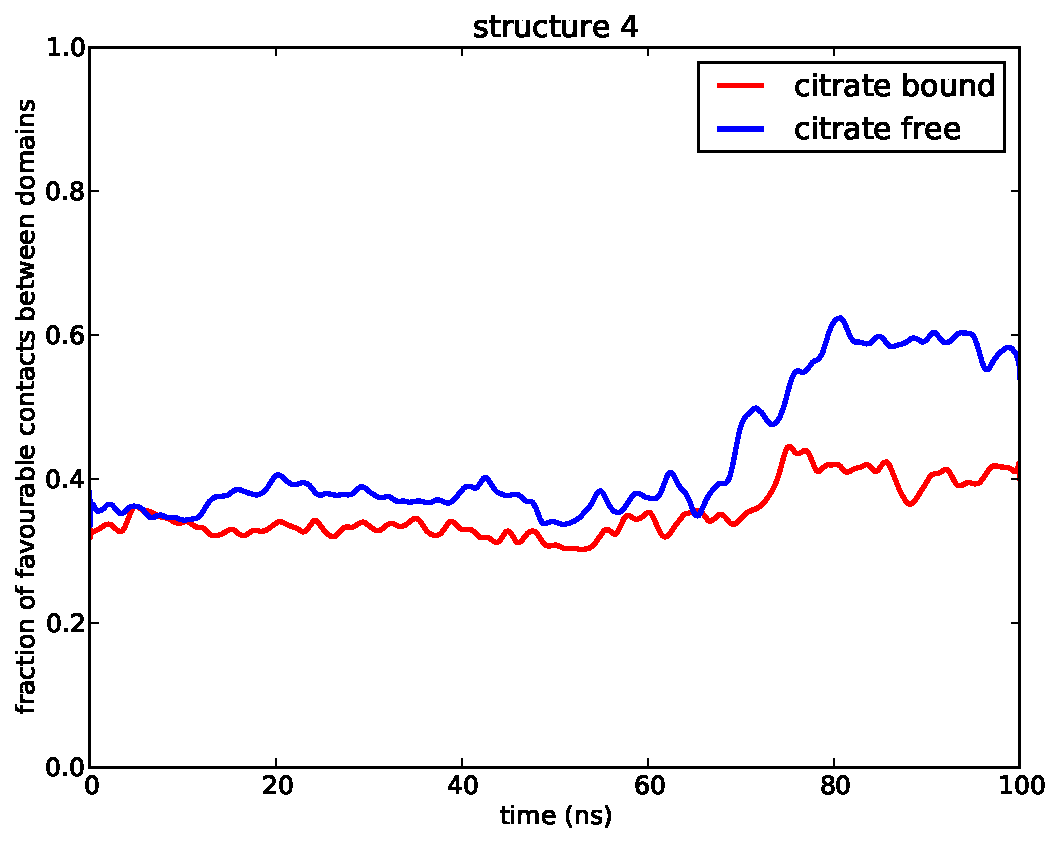
\includegraphics[width=0.85\textwidth]{figures/Complex_hydrophobic_core/favourable_cont_structure4.pdf}  
        \end{figure}       

    \end{columns}   
    
\end{frame}       

% ============================================================================ %

\begin{frame}
    \frametitle{Results}
    \framesubtitle{Fusion Protein MD -- Hydrophobic Contacts}  

    \vspace{0.06\topmargin}

    \begin{columns}[t]
        \column{.5\linewidth}
        \vspace{-4ex}
        \begin{figure}
            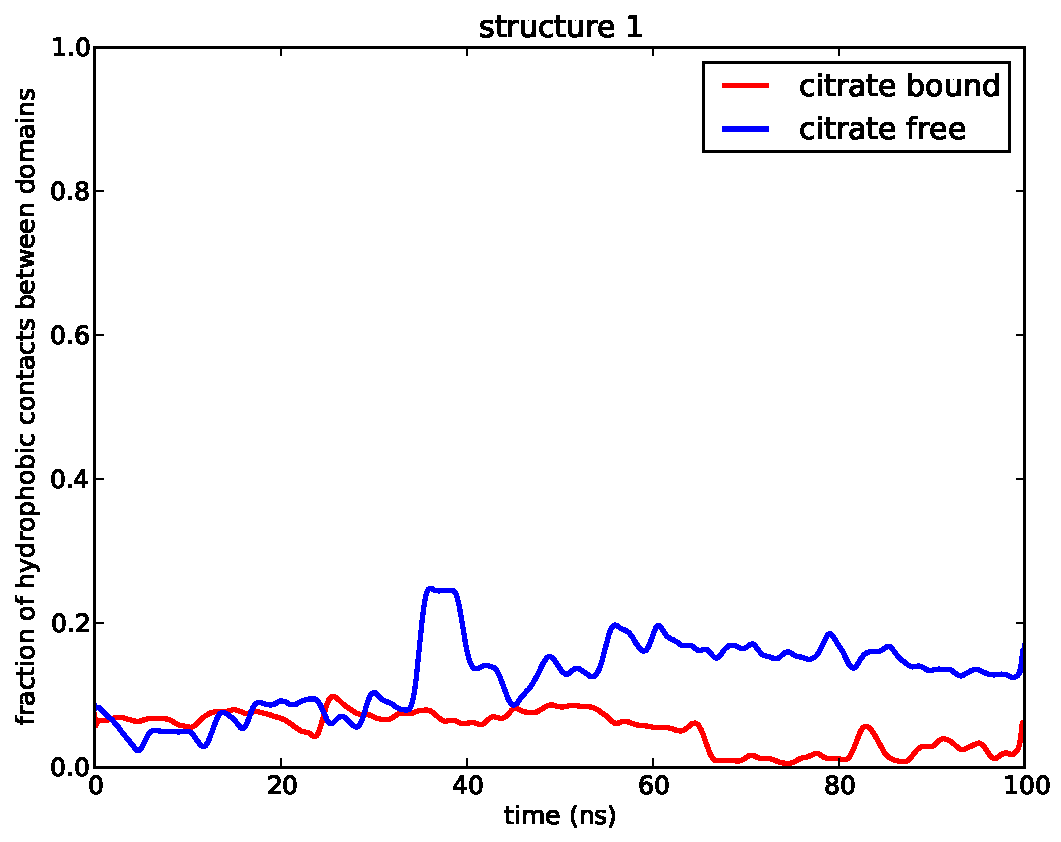
\includegraphics[width=0.85\textwidth]{figures/Complex_hydrophobic_core/hydrophobic_cont_structure1.pdf}  
        \end{figure}      
        \vspace{-5ex}
        \begin{figure}
            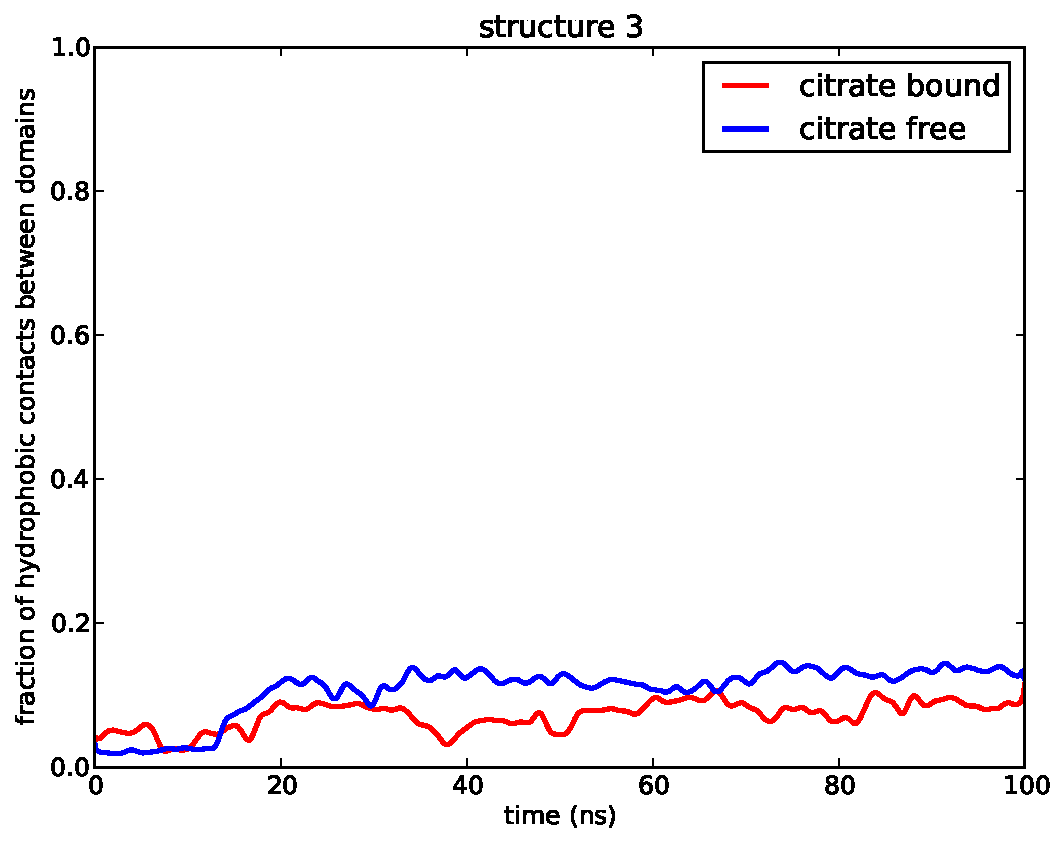
\includegraphics[width=0.85\textwidth]{figures/Complex_hydrophobic_core/hydrophobic_cont_structure3.pdf}  
        \end{figure}       

        \column{.5\linewidth}
        \vspace{-4ex}
        \begin{figure}
            \includegraphics[width=0.85\textwidth]{figures/Complex_hydrophobic_core/hydrophobic_cont_structure2.pdf}  
        \end{figure}      
        \vspace{-5ex}
        \begin{figure}
            \includegraphics[width=0.85\textwidth]{figures/Complex_hydrophobic_core/hydrophobic_cont_structure4.pdf}  
        \end{figure}       

    \end{columns}   
    
\end{frame}       
 
% ============================================================================ %

\end{document}
